\documentclass{beamer}

% xcolor and define colors -------------------------
\usepackage{xcolor}

% https://www.viget.com/articles/color-contrast/
\definecolor{purple}{HTML}{5601A4}
\definecolor{navy}{HTML}{0D3D56}
\definecolor{ruby}{HTML}{9a2515}
\definecolor{alice}{HTML}{107895}
\definecolor{daisy}{HTML}{EBC944}
\definecolor{coral}{HTML}{F26D21}
\definecolor{kelly}{HTML}{829356}
\definecolor{cranberry}{HTML}{E64173}
\definecolor{jet}{HTML}{131516}
\definecolor{asher}{HTML}{555F61}
\definecolor{slate}{HTML}{314F4F}

% Mixtape Sessions
\definecolor{picton-blue}{HTML}{00b7ff}
\definecolor{violet-red}{HTML}{ff3881}
\definecolor{sun}{HTML}{ffaf18}
\definecolor{electric-violet}{HTML}{871EFF}

% Main theme colors
\definecolor{accent}{HTML}{00b7ff}
\definecolor{accent2}{HTML}{871EFF}
\definecolor{gray100}{HTML}{f3f4f6}
\definecolor{gray800}{HTML}{1F292D}


% Beamer Options -------------------------------------

% Background
\setbeamercolor{background canvas}{bg = white}

% Change text margins
\setbeamersize{text margin left = 15pt, text margin right = 15pt} 

% \alert
\setbeamercolor{alerted text}{fg = accent2}

% Frame title
\setbeamercolor{frametitle}{bg = white, fg = jet}
\setbeamercolor{framesubtitle}{bg = white, fg = accent}
\setbeamerfont{framesubtitle}{size = \small, shape = \itshape}

% Block
\setbeamercolor{block title}{fg = white, bg = accent2}
\setbeamercolor{block body}{fg = gray800, bg = gray100}

% Title page
\setbeamercolor{title}{fg = gray800}
\setbeamercolor{subtitle}{fg = accent}

%% Custom \maketitle and \titlepage
\setbeamertemplate{title page}
{
    %\begin{centering}
        \vspace{20mm}
        {\Large \usebeamerfont{title}\usebeamercolor[fg]{title}\inserttitle}\\
        {\large \itshape \usebeamerfont{subtitle}\usebeamercolor[fg]{subtitle}\insertsubtitle}\\ \vspace{10mm}
        {\insertauthor}\\
        {\color{asher}\small{\insertdate}}\\
    %\end{centering}
}

% Table of Contents
\setbeamercolor{section in toc}{fg = accent!70!jet}
\setbeamercolor{subsection in toc}{fg = jet}

% Button 
\setbeamercolor{button}{bg = accent}

% Remove navigation symbols
\setbeamertemplate{navigation symbols}{}

% Table and Figure captions
\setbeamercolor{caption}{fg=jet!70!white}
\setbeamercolor{caption name}{fg=jet}
\setbeamerfont{caption name}{shape = \itshape}

% Bullet points

%% Fix left-margins
\settowidth{\leftmargini}{\usebeamertemplate{itemize item}}
\addtolength{\leftmargini}{\labelsep}

%% enumerate item color
\setbeamercolor{enumerate item}{fg = accent}
\setbeamerfont{enumerate item}{size = \small}
\setbeamertemplate{enumerate item}{\insertenumlabel.}

%% itemize
\setbeamercolor{itemize item}{fg = accent!70!white}
\setbeamerfont{itemize item}{size = \small}
\setbeamertemplate{itemize item}[circle]

%% right arrow for subitems
\setbeamercolor{itemize subitem}{fg = accent!60!white}
\setbeamerfont{itemize subitem}{size = \small}
\setbeamertemplate{itemize subitem}{$\rightarrow$}

\setbeamertemplate{itemize subsubitem}[square]
\setbeamercolor{itemize subsubitem}{fg = jet}
\setbeamerfont{itemize subsubitem}{size = \small}







% Links ----------------------------------------------

\usepackage{hyperref}
\hypersetup{
  colorlinks = true,
  linkcolor = accent2,
  filecolor = accent2,
  urlcolor = accent2,
  citecolor = accent2,
}


% Line spacing --------------------------------------
\usepackage{setspace}
\setstretch{1.2}


% \begin{columns} -----------------------------------
\usepackage{multicol}


% Fonts ---------------------------------------------
% Beamer Option to use custom fonts
\usefonttheme{professionalfonts}

% \usepackage[utopia, smallerops, varg]{newtxmath}
% \usepackage{utopia}
\usepackage[sfdefault,light]{roboto}

% Small adjustments to text kerning
\usepackage{microtype}



% Remove annoying over-full box warnings -----------
\vfuzz2pt 
\hfuzz2pt


% Table of Contents with Sections
\setbeamerfont{myTOC}{series=\bfseries, size=\Large}
\AtBeginSection[]{
        \frame{
            \frametitle{Roadmap}
            \tableofcontents[current]   
        }
    }


% Tables -------------------------------------------
% Tables too big
% \begin{adjustbox}{width = 1.2\textwidth, center}
\usepackage{adjustbox}
\usepackage{array}
\usepackage{threeparttable, booktabs, adjustbox}
    
% Fix \input with tables
% \input fails when \\ is at end of external .tex file
\makeatletter
\let\input\@@input
\makeatother

% Tables too narrow
% \begin{tabularx}{\linewidth}{cols}
% col-types: X - center, L - left, R -right
% Relative scale: >{\hsize=.8\hsize}X/L/R
\usepackage{tabularx}
\newcolumntype{L}{>{\raggedright\arraybackslash}X}
\newcolumntype{R}{>{\raggedleft\arraybackslash}X}
\newcolumntype{C}{>{\centering\arraybackslash}X}

% Figures

% \imageframe{img_name} -----------------------------
% from https://github.com/mattjetwell/cousteau
\newcommand{\imageframe}[1]{%
    \begin{frame}[plain]
        \begin{tikzpicture}[remember picture, overlay]
            \node[at = (current page.center), xshift = 0cm] (cover) {%
                \includegraphics[keepaspectratio, width=\paperwidth, height=\paperheight]{#1}
            };
        \end{tikzpicture}
    \end{frame}%
}

% subfigures
\usepackage{subfigure}


% Highlight slide -----------------------------------
% \begin{transitionframe} Text \end{transitionframe}
% from paulgp's beamer tips
\newenvironment{transitionframe}{
    \setbeamercolor{background canvas}{bg=accent!40!black}
    \begin{frame}\color{accent!10!white}\LARGE\centering
}{
    \end{frame}
}


% Table Highlighting --------------------------------
% Create top-left and bottom-right markets in tabular cells with a unique matching id and these commands will outline those cells
\usepackage[beamer,customcolors]{hf-tikz}
\usetikzlibrary{calc}
\usetikzlibrary{fit,shapes.misc}

% To set the hypothesis highlighting boxes red.
\newcommand\marktopleft[1]{%
    \tikz[overlay,remember picture] 
        \node (marker-#1-a) at (0,1.5ex) {};%
}
\newcommand\markbottomright[1]{%
    \tikz[overlay,remember picture] 
        \node (marker-#1-b) at (0,0) {};%
    \tikz[accent!80!jet, ultra thick, overlay, remember picture, inner sep=4pt]
        \node[draw, rectangle, fit=(marker-#1-a.center) (marker-#1-b.center)] {};%
}

\usepackage{breqn} % Breaks lines

\usepackage{amsmath}
\usepackage{mathtools}

\usepackage{pdfpages} % \includepdf

\usepackage{listings} % R code
\usepackage{verbatim} % verbatim

% Video stuff
\usepackage{media9}

% packages for bibs and cites
\usepackage{natbib}
\usepackage{har2nat}
\newcommand{\possessivecite}[1]{\citeauthor{#1}'s \citeyearpar{#1}}
\usepackage{breakcites}
\usepackage{alltt}

% tikz
\usepackage{tikz}
\usepackage{pgfplots}
\usetikzlibrary{calc, positioning, decorations.pathreplacing, arrows.meta, intersections}
\pgfdeclarelayer{bg}
\pgfdeclarelayer{back}
\pgfdeclarelayer{fg}
\pgfsetlayers{bg,main,fg,back}
\usetikzlibrary{shapes,arrows}

% Setup math operators
\DeclareMathOperator{\E}{E} \DeclareMathOperator{\tr}{tr} \DeclareMathOperator{\se}{se} \DeclareMathOperator{\I}{I} \DeclareMathOperator{\sign}{sign} \DeclareMathOperator{\supp}{supp} \DeclareMathOperator{\plim}{plim}
\DeclareMathOperator*{\dlim}{\mathnormal{d}\mkern2mu-lim}
\newcommand\independent{\protect\mathpalette{\protect\independenT}{\perp}}
   \def\independenT#1#2{\mathrel{\rlap{$#1#2$}\mkern2mu{#1#2}}}
\newcommand*\colvec[1]{\begin{pmatrix}#1\end{pmatrix}}

\newcommand{\myurlshort}[2]{\href{#1}{\textcolor{gray}{\textsf{#2}}}}


\begin{document}

\imageframe{./lecture_includes/mixtape_ci_cover.png}


% ---- Content ----


\section{Introduction to course}

\begin{frame}{Welcome to Mixtape Sessions!}

  \begin{itemize}
    \item Mixtape Sessions is an educational platform designed to ``democratize causal inference'' at all levels by helping bridging people with teachers
    \item This workshop, and others like it, are important because of how important causal inference is and how in demand it has become and how erratically spread across disciplines the material is taught if at all
  \end{itemize}

\end{frame}

\begin{frame}{Why Mixtape Sessions}

  \begin{itemize}

    \item Scott Cunningham, Ben Williams Professor of Economics, Baylor University 
    \item Not an econometrician; just your run of the mill typical applied microeconomist
    \item Workshop is about the science but also the art of causal inference (as is the broader Mixtape Sessions platform)

  \end{itemize}

\end{frame}

\begin{frame}{Class goals}

  \begin{enumerate}
    \item \textbf{Confidence}: You will feel like you have a good understanding of design-based causal inference by the end such that it doesn't feel so mysterious or intimidating
    \item \textbf{Comprehension}: You will have learned a lot both conceptually but also in various specifics, particularly with regards to issues around identification and estimation
    \item \textbf{Competency}: you will have had some experience working together implementing these methods using code in Stata and R, syntax, possession of programs, knowledge of packages
  \end{enumerate}

\end{frame}

\begin{frame}{4-day Causal Inference Workshop}

  \begin{itemize}
    \item Our workshop together is 4-days, 8am to 5pm CST, with 15 min breaks on the hour and a 1-hour lunch break at 12:00PM CST
    \item It will mix exposition, discussion of papers, coding exercises and discussion as best as I can
    \item It's essentially a semester's worth of material
  \end{itemize}

\end{frame}

\begin{frame}{Causal Inference table of contents}
  \centering
  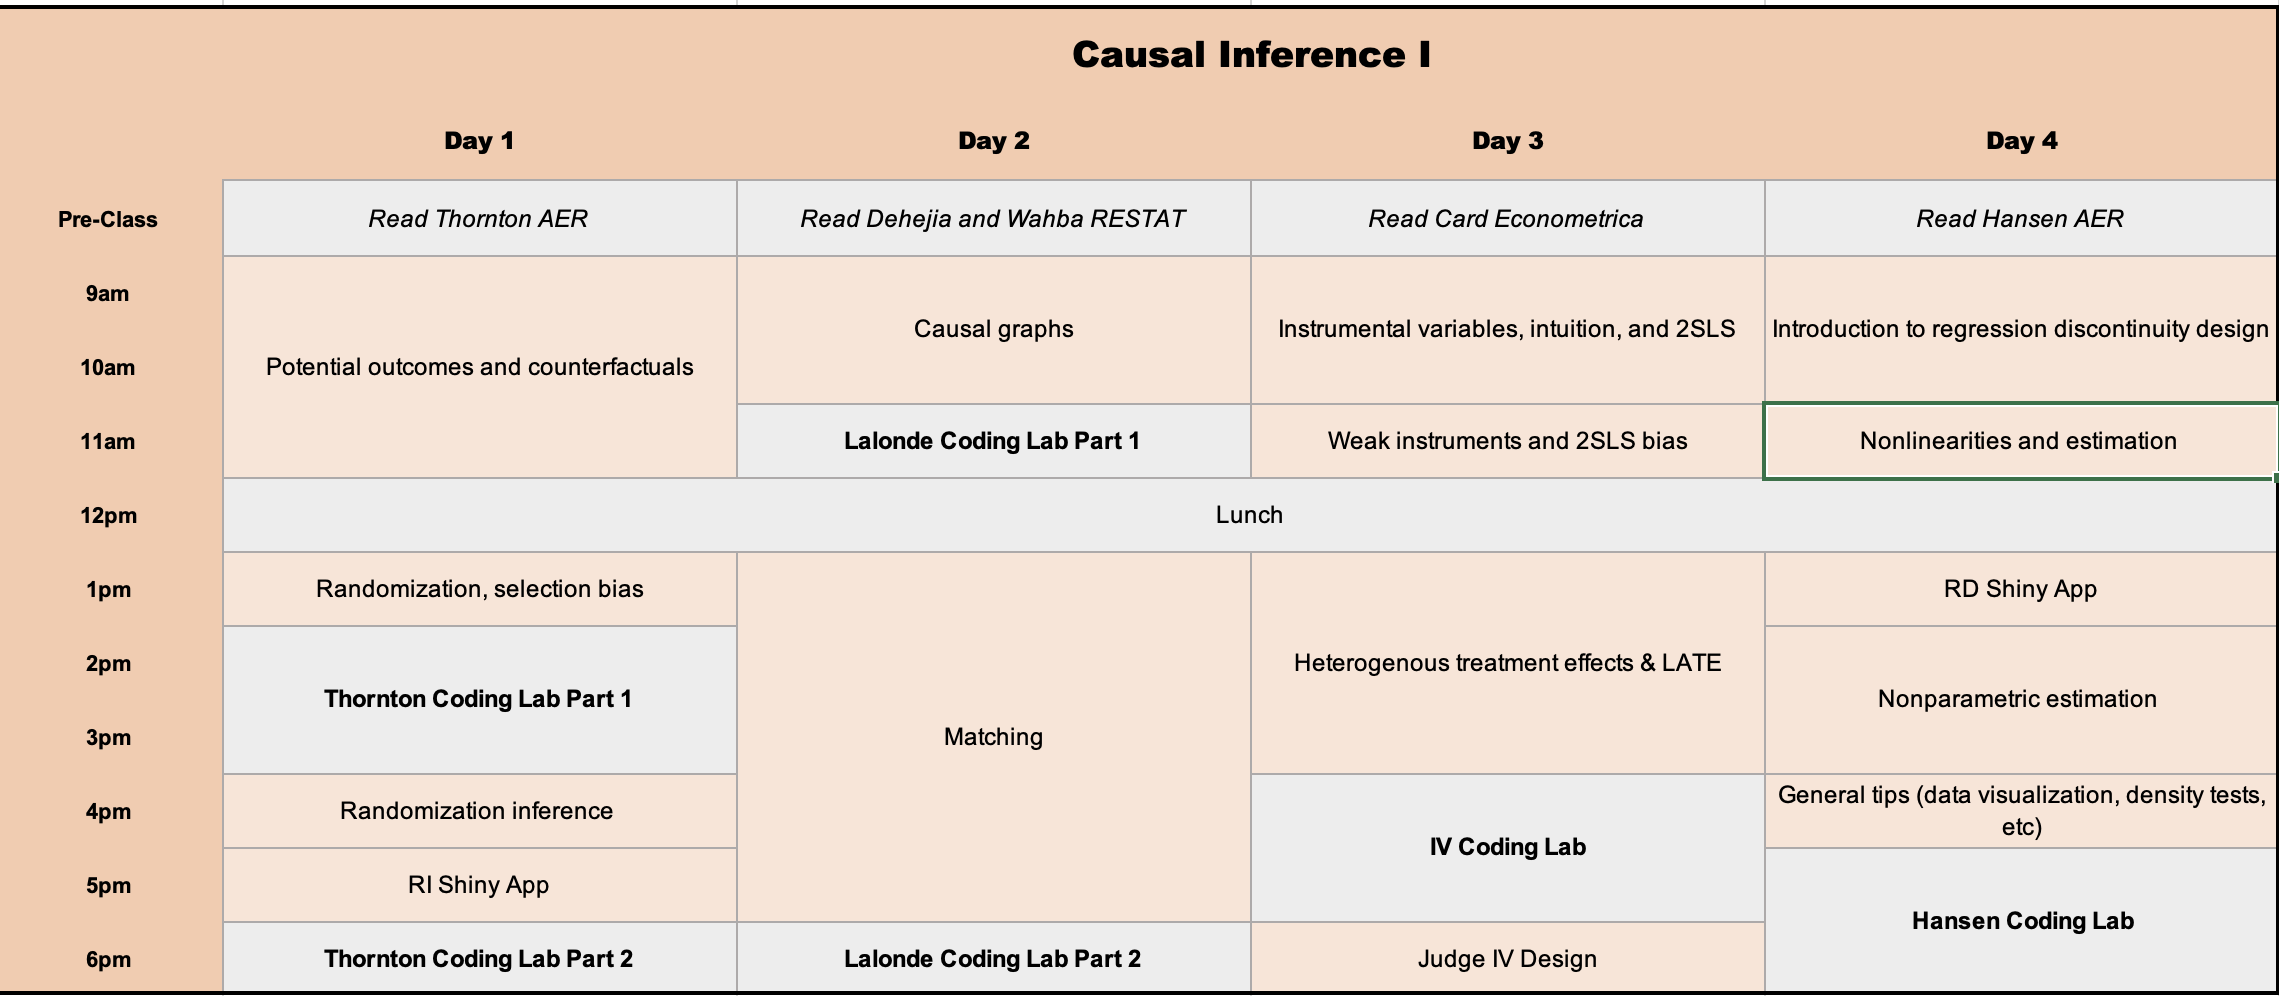
\includegraphics[scale=0.5,height=6.5cm, width=10cm]{./lecture_includes/part1}
\end{frame}

%\begin{frame}{Causal Inference Part 2}
%  \centering
%  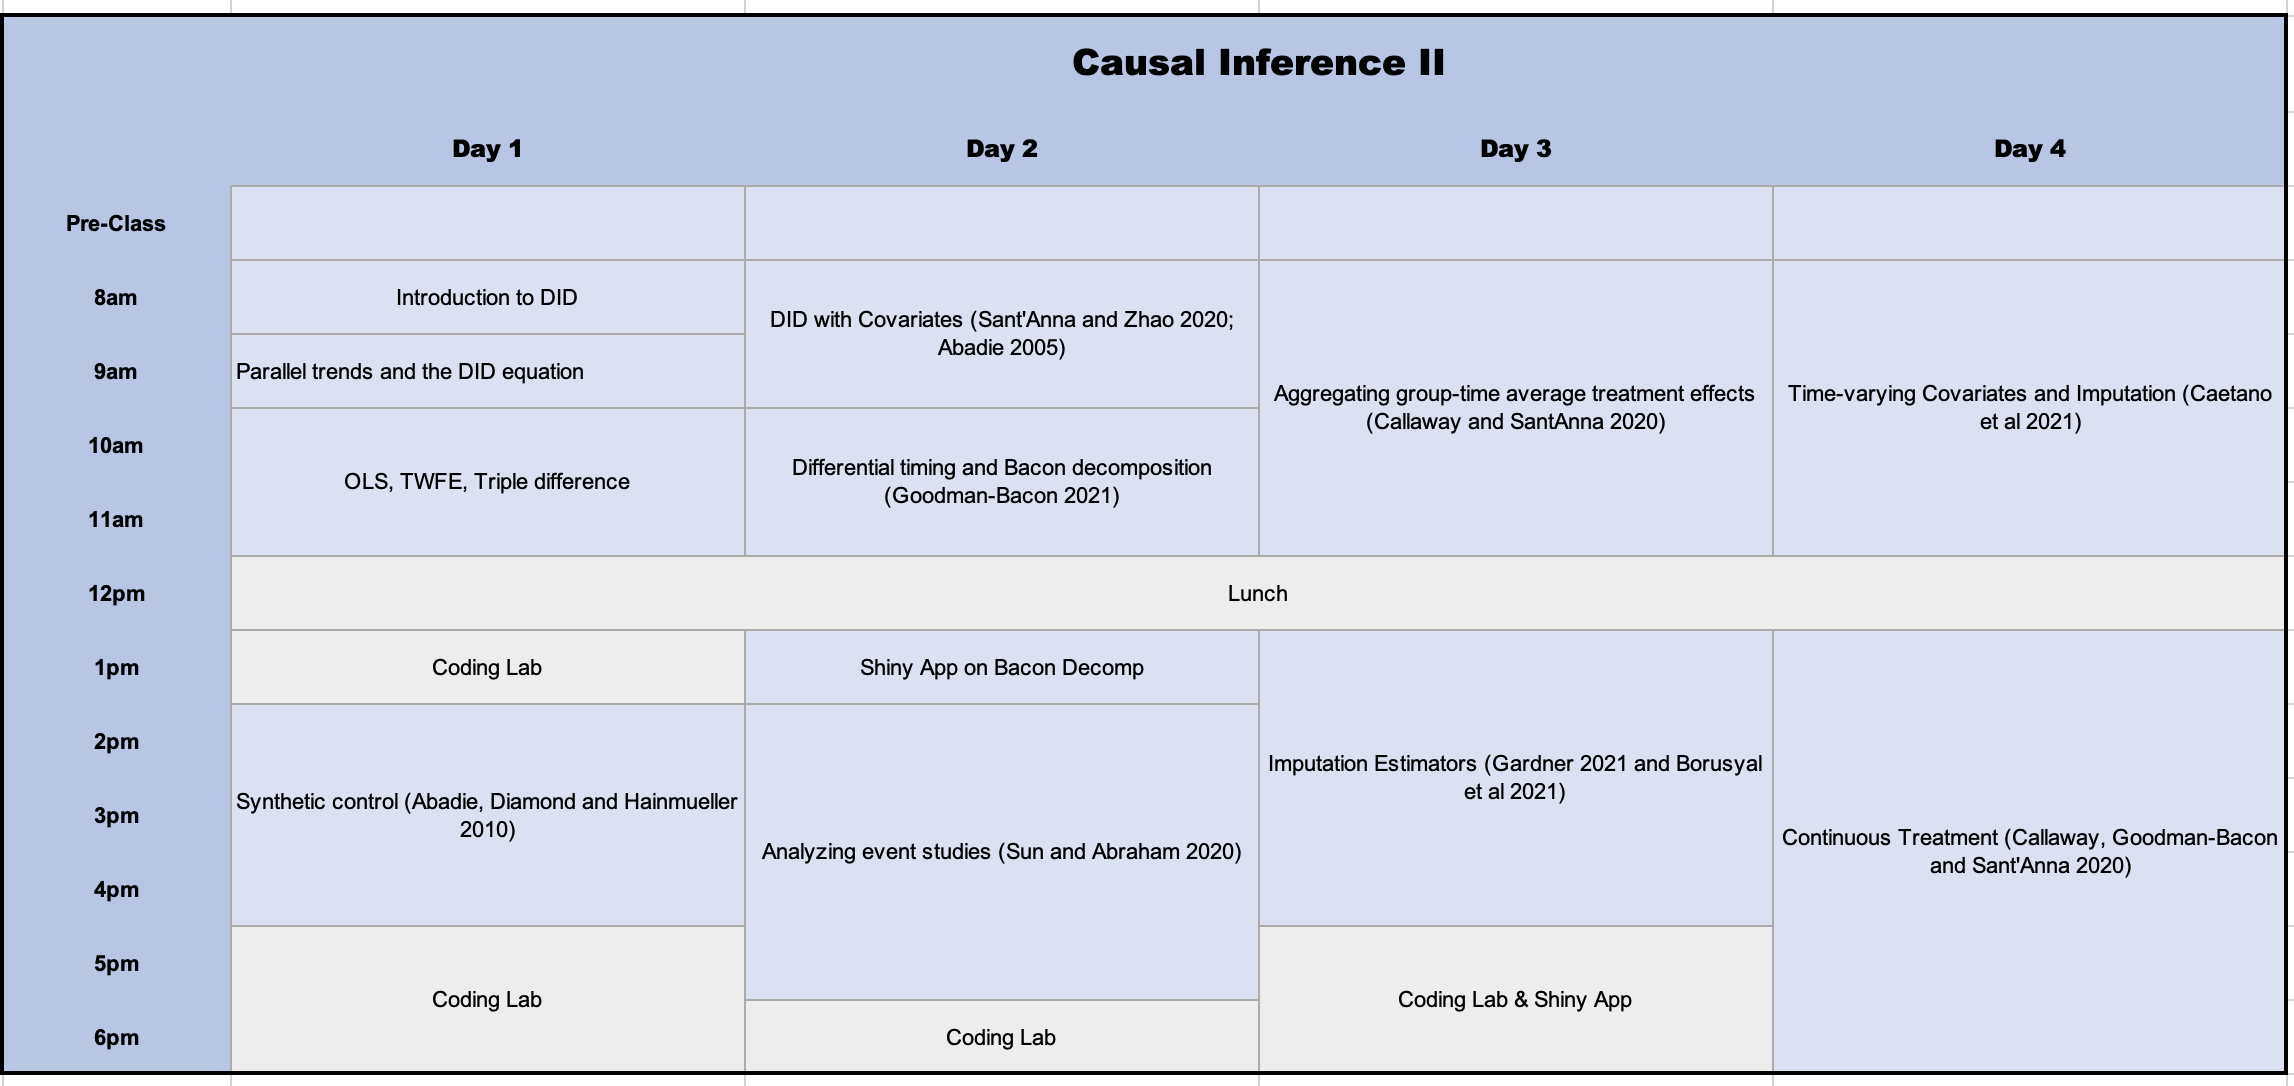
\includegraphics[scale=0.5,height=6.5cm, width=10cm]{./lecture_includes/part2}
%  \url{https://www.mixtapesessions.io/session/ci_II_aug20}
%\end{frame}




%\begin{frame}{Github repo}
%
%  \begin{itemize}
%    \item We will communicate with one another regularly in the Discord channel and I will always be monitoring it
%    \item I will be distributing things to you, like code and slides, via the github repo: \url{github.com/Mixtape-Sessions/Causal-Inference-1}
%    \item Each lecture will be recorded and then uploaded to Vimeo as a password protected file that you'll have access to into perpetutity
%  \end{itemize}

%\end{frame}

\begin{frame}{Workshop (Part 1) Topics}

  \begin{enumerate}
    \item Foundations: Day 1
    \item Graphs and Selection on Observables: Day 2
    \item Instrumental Variables: Day 3
    \item Regression Discontinuity Design: Day 4
  \end{enumerate}

\end{frame}


\subsection{Brief history of design-based causal inference}



\begin{frame}{Credibility Problem Within Empirical Economics}

  \begin{itemize}
  \item Tremendous turmoil in applied economics in late 1970s and early 1980s
  \item Several high profile papers found serious credibility problems in many applied studies, particularly those using macro data
  \item This criticism eventually turned to labor economics which was vulnerable because of its early adoption of rich micro data and microeconometric methods (``Pioneers take arrows in the back'')
  \end{itemize}

\end{frame}



\begin{frame}{Lewis 1986 book}

\begin{quote}
``After reviewing virtually every study since 1963, Lewis reached the awkward conclusion that simple OLS of union wage effects were more useful and reliable than those based on IV or endogenous selection approaches. The problem, in his view, was that researchers used \emph{arbitrary} and \emph{unsupported assumptions} to identify their models with little or no concern for the validity of their assumptions or the implications of their findings. This criticism was particularly salient because many of the new methods had been tested initially on the union wage effect question (e.g., Lee 1978).'' -- Card (2022)
\end{quote}

\end{frame}

\begin{frame}{Replication problems}

\begin{itemize}
\item Deward, Thursby and Anderson (1986) suggest that applied estimates can't be replicated partly bc many authors won't share their data or their programs
\item They tried to replicate the papers at the JMCB journal between 1980 and 1984 (there was a data sharing agreement in 1982 and 1/4 authors still won't respond to request; before that 2/3 failed to respond)
\item Only 2 of 9 papers could be reproduced exactly; 5 had substantial errors
\end{itemize}

\end{frame}

\begin{frame}{Take the con out of econometrics}

\begin{itemize}
\item Famous paper by Ed Leamer -- ``Take the con out of econometrics''
\item He says in Hendry, Leamer and Poirier (1990), ``we don't take empirical work seriously in economics. It's not the source by which economists accumulate their opinions, by and large.''
\item Hits hard at Princeton's Industrial Relations Section where Card, Ashenfelter, Krueger, Angrist, Lalonde, and more are. They seek to fix this
\end{itemize}

\end{frame}

\begin{frame}{Princeton IRS Model}

\begin{itemize}
\item Ashenfelter 1970s work in government focuses on extreme self-selection into job trainings programs (``Ashenfelter dip''); Ashenfelter and Card (1985) note longitudinal studies are not designed for this 
\item Princeton Industrial Relations Section Model: more transparency, more credible ``research design'' that make explicit sources of identification and work hard to verify the legitimacy of that source
\item Krueger notes that he would read NEJM and they'd often include a short description of the study's ``research design''
\end{itemize}

\end{frame}

\begin{frame}{Natural experiments}

\begin{itemize}
\item Richard Freeman had been pushing for natural experiments for years -- ``big shocks'' like federal minimum wages in Puerto Rico
\item Card really pushes this early on 
	\begin{itemize}
	\item Immigration labor supply shifts from the Mariel Boatlift paper (Card 1990); 
	\item Minimum wage increases from neighboring state comparisons (Card and Krueger 1994)
	\end{itemize}
\item Steven Levitt seems instrumental in the late 1990s for bringing natural experiments and this labor economics approach to crime, more or less cleaning house; also very good abt sharing data and programs

\end{itemize}

\end{frame}

\subsection{Design's Growing Influence}

\begin{frame}{Theory's role}

\begin{itemize}
\item Economists write models to help them understand the world
\item Economists also use those models to guide their empirical work
\item But the connection between those two steps has not always been done the same; let's review as this framework can help give you the big picture
\end{itemize}

\end{frame}


\begin{frame}{Design vs Model}

  \begin{itemize}
    \item \textbf{Model}: Causality exists within the framework of a theory that says ``D causes Y'' (e.g., Heckman)
    \item \textbf{Design}: Causality is design-based and can be discerned with \emph{physical} manipulation of a treatment $D$ (e.g., Rubin, Holland)
  \end{itemize}
\end{frame}


\begin{frame}{Approximating models}

  \begin{enumerate}
    \item[1. ] \textbf{Approximating models}: Consumer demand, labor supply models (e.g., Mincer 1958; 1974)
          \begin{itemize}
            \item Theory implies $y_i=f_i(x_i)$ with restrictions on $f_i$ (e.g., concavity)
            \item Researcher estimates a simpler version $$y_i = \alpha + x_i \beta + \varepsilon_i$$
          \end{itemize}
  \end{enumerate}

\end{frame}

\begin{frame}{Exact models}

  \begin{enumerate}
    \item[2. ] \textbf{Exact models}: Models gives us all causes (``complete DGP'')
          \begin{itemize}
            \item More structural approach to identification, less focused on physical assignment of treatments
            \item Estimate model parameters and distribution of heterogeneity
            \item Functional form, useful for welfare analysis
          \end{itemize}
  \end{enumerate}

\end{frame}

\begin{frame}{Working model}

  \begin{enumerate}
    \item[3. ] \textbf{Working model}: Called reduced form, program evaluation, more like Princeton's IRS model
          \begin{itemize}
            \item Model formulates questions, intuition, but does not necessarily assist with identification
            \item Focus is on physical assignment of treatments not on modeling assumptions
            \item Extreme focus on verifying the assumptions through placebos, falsifications, checks for identifying assumptions throughout
          \end{itemize}
  \end{enumerate}

  \bigskip

Models are useful, but not necessarily \emph{used}, the way they are in structural approaches

\end{frame}


\begin{frame}{Topics broaden}

  Dependence on the model vs freed from the model for causal inference increases topics
  \begin{itemize}
    \item \textbf{Design}: Anything goes, ``economics is what economists study'', happiness, fringe stuff (e.g., sex work) (opening up topics)
    \item \textbf{Model}: Neoclassical topics due to needing agreed upon models (limiting topics)
  \end{itemize}

\end{frame}

\begin{frame}{Strengths of design}

\begin{itemize}
\item Approaches are oftentimes easier to explain; identification (historically a mathematical term) becomes synonymous with research design (Imbens and Angrist 1994)
\item Precise research designs, as we will see, make it much easier to evaluate the core assumptions of the model (like employing event studies in a diff-in-diff)
\item Designs become portable -- we can repeat these approaches in other settings (which is in many ways what this class is doing)
\end{itemize}

\end{frame}

\begin{frame}{Weaknesses}

\begin{itemize}
\item Limits the questions we can answer oftentimes 
	\begin{itemize}
	\item It's very backwards looking (may be a strength insofar as it's conservative)
	\item Lacks generalizability
	\end{itemize}
\item Listen to Petra Todd describe these weaknesses \url{https://youtu.be/m1Mpc7-b-1I?t=2776}

\end{itemize}

\end{frame}


\section{Potential outcomes}

\subsection{Naive correlation}

\begin{frame}{What is causality?}

  \begin{quote}
    ``Causation is something that makes a difference, and the difference it makes must be a difference from what would have happened without it.'' -- David Lewis (philosopher)
  \end{quote}

  \bigskip
  Key idea $\rightarrow$ counterfactual. Counterfactuals are neither past nor future.  They are alternative histories created by thought experiments but we use them as framing devices to decipher causality in our timeline

  \bigskip

  Causal inference is also fundamentally practically because if we know causality, then we can also know not only the past, but also the future (policy)

\end{frame}

\begin{frame}{Different types of prediction}

  \begin{columns}
    \column{0.48\linewidth}
    \centering
    \textbf{Traditional prediction}
    \begin{itemize}
      \item Traditional prediction seeks to detect patterns in data and fit functional relationships between variables with a high degree of accuracy
      \item ``Does this person have heart disease?'', ``How many books will I sell?''
      \item It is not predictions of what effect a choice will have, though
    \end{itemize}
    \column{0.48\linewidth}
    \centering
    \textbf{Causal inference}
    \begin{itemize}
      \item Causal inference is also a type of prediction, but it's a prediction of a \emph{counterfactual} associated with a particular \emph{choice taken}
      \item Causal inference takes that predicted (or imputed) counterfactual and constructs a causal effect that we hope tells us about a future in the event of a similar choice taken
    \end{itemize}
  \end{columns}
\end{frame}


\begin{frame}{Identification problem}
  \centering
  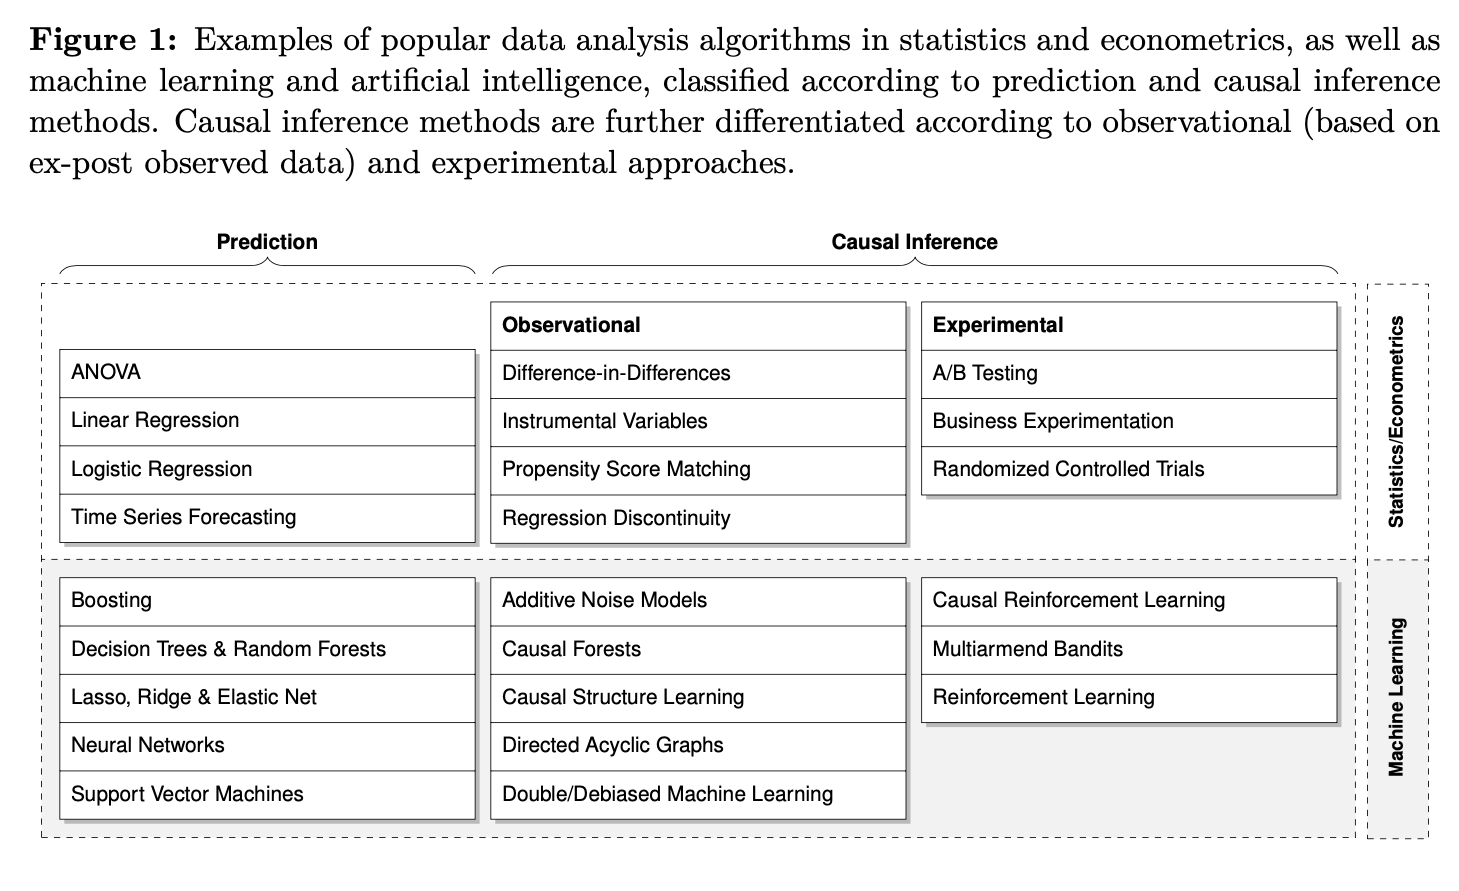
\includegraphics[scale=0.5,height=6.5cm, width=10cm]{./lecture_includes/prediction_causality.png}
\end{frame}




\begin{frame}{Introduction to Counterfactuals}

  \begin{itemize}
    \item Aliens come and orbit earth, see people dying in hospitals and conclude ``doctors are hurting people''
    \item They kill the doctors, unplug patients from machines, throw open the doors -- many patients inexplicably die
    \item \emph{We are the aliens in our research}
  \end{itemize}

\end{frame}

\begin{frame}{\#1: Correlation and causality are different}

  Causal is one unit, correlation is many units
  \begin{itemize}
    \item Causal question: ``If a doctor puts a patient on a ventilator (D), will her covid symptoms (Y) improve?''
    \item Correlation question:  $$\frac{Cov(D,Y)}{\sqrt{Var_D}\sqrt{{Var_Y}}}$$
  \end{itemize}

\end{frame}


\begin{frame}{\#2: Coming first may not mean causality!}

  \begin{itemize}
    \item Every morning the rooster crows and then the sun rises
    \item Did the rooster cause the sun to rise? Or did the sun cause the rooster to crow?
    \item What if cat killed the rooster?
    \item \emph{Post hoc ergo propter hoc}: ``after this, therefore, because of this''
  \end{itemize}

\end{frame}

\begin{frame}[plain]

  \begin{figure}
    \centering
    \includegraphics[scale=0.04]{./lecture_includes/scottboat.jpg}
  \end{figure}

\end{frame}

\begin{frame}{\#3: No correlation does not mean no causality!}

  \begin{itemize}
    \item A sailor sails her sailboat across a lake
    \item Wind blows, and she perfectly counters by turning the rudder
    \item The same aliens observe from space and say ``Look at the way she's moving that rudder back and forth but going in a straight line.  That rudder is broken.'' So they send her a new rudder
    \item They're wrong but why are they wrong? There is, after all, no correlation
    \item Example: Fed and open market operations
  \end{itemize}

\end{frame}

\subsection{Potential outcomes notation}

\begin{frame}{What is causality?}

  \begin{quote}
    ``Causation is something that makes a difference, and the difference it makes must be a difference from what would have happened without it.'' -- David Lewis (philosopher)
  \end{quote}

  \bigskip
  Key idea $\rightarrow$ counterfactual. Counterfactuals are neither past nor future.  They are alternative histories created by thought experiments but we use them as framing devices to decipher causality in our timeline

  \bigskip

  Causal inference is also fundamentally practically because if we know causality, then we can also know not only the past, but also the future (policy)

\end{frame}

\begin{frame}{Different types of prediction}

  \begin{columns}
    \column{0.48\linewidth}
    \centering
    \textbf{Traditional prediction}
    \begin{itemize}
      \item Traditional prediction seeks to detect patterns in data and fit functional relationships between variables with a high degree of accuracy
      \item ``Does this person have heart disease?'', ``How many books will I sell?''
      \item It is not predictions of what effect a choice will have, though
    \end{itemize}
    \column{0.48\linewidth}
    \centering
    \textbf{Causal inference}
    \begin{itemize}
      \item Causal inference is also a type of prediction, but it's a prediction of a \emph{counterfactual} associated with a particular \emph{choice taken}
      \item Causal inference takes that predicted (or imputed) counterfactual and constructs a causal effect that we hope tells us about a future in the event of a similar choice taken
    \end{itemize}
  \end{columns}
\end{frame}


\begin{frame}{Identification problem}
  \centering
  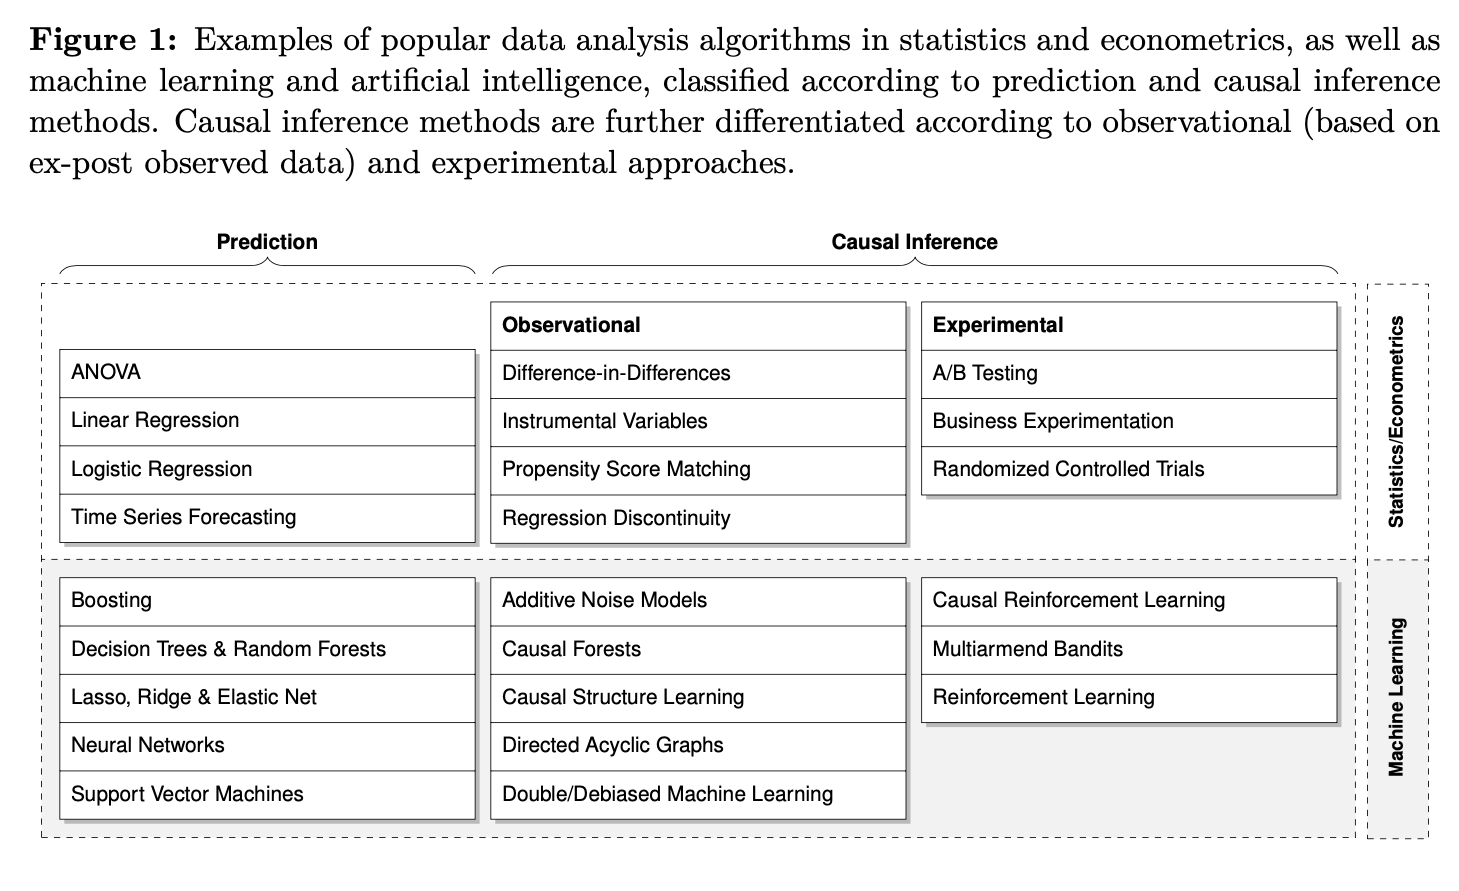
\includegraphics[scale=0.5,height=6.5cm, width=10cm]{./lecture_includes/prediction_causality.png}
\end{frame}



\begin{frame}{Potential outcomes}

\begin{itemize}
\item Conceptual framework for design based causal inference is counterfactual reasoning
\item Counterfactual modeling becomes linked to potential outcomes models with Don Rubin 1970s work on propensity scores
\item Potential outcomes notation was created by Jerzy Neyman (1923) and led Ronald Fisher (1925) to suggest RCTs
\item Huge push by Donald Rubin, a Neyman ``grandson'', in the 1970s and 1980s with Paul Rosenbaum on the propensity score
\item Guido Imbens, a Rubin coauthor, notes that it was crucial to his work on IV with Angrist, but it may even have made that work more appealing \emph{outside economics}
\url{https://youtu.be/cm8V65AS5iU?t=1097}

\end{itemize}

\end{frame}




\begin{frame}{Potential outcomes notation}

  \begin{itemize}
    \item Let the treatment be a binary variable: $$D_{i,t} =\begin{cases} 1 \text{ if hospitalized at time $t$} \\ 0 \text{ if not hospitalized at time $t$} \end{cases}$$where $i$ indexes an individual observation, such as a person
  \end{itemize}
\end{frame}

\begin{frame}{Potential outcomes notation}

  \begin{itemize}
    \item Potential outcomes: $$Y_{i,t}^j =\begin{cases} 1 \text{ health if hospitalized at time $t$} \\ 0 \text{ health if not hospitalized at time $t$} \end{cases}$$where $j$ indexes a counterfactual state of the world
  \end{itemize}
\end{frame}


\begin{frame}{Realized vs potential outcomes}

  \begin{itemize}
    \item Potential outcomes $Y^1$ are not the realized outcomes $Y$ either conceptually or notationally
    \item Potential outcomes are hypothetical states of the world but realized outcomes are \emph{ex post} the observed outcomes we have in our data due to treatment assignment
    \item This distinction is subtle, creates challenges at the introductory stage, it isn't how econometrics was historically taught, except for at the very beginning; again Imbens on this \url{https://youtu.be/cm8V65AS5iU?t=1175}
  \end{itemize}
\end{frame}



\begin{frame}{Important definitions}


  \begin{columns}[t]
    \scriptsize
    \column{.45\textwidth}

    \begin{block}{Definition 1: Individual treatment effect}
      The individual treatment effect,  $\delta_i$, equals $Y_i^1-Y_i^0$
    \end{block}
    \begin{block}{Definition 3: Fundamental problem of causal inference}
      If you need both potential outcomes to know causality with certainty, then since it is impossible to observe both $Y_i^1$ and $Y_i^0$ for the same individual, $\delta_i$, is \emph{unknowable}.
    \end{block}
    \column{.45\textwidth}
    \begin{block}{Definition 2: Switching equation}
      An individual's observed health outcomes, $Y$, is determined by treatment assignment, $D_i$, and corresponding potential outcomes:
      \begin{eqnarray*}
        Y_i& = D_iY^1_i+(1-D_i)Y^0_i& \\
        Y_i& = \begin{cases}
          Y^1_i\text{ if }D_i=1 \\
          Y^0_i\text{ if }D_i=0
        \end{cases}
      \end{eqnarray*}
    \end{block}

  \end{columns}
\end{frame}

\begin{frame}{Missing data problem}

  \begin{itemize}
    \item Causal inference is fundamentally a missing data problem requiring prediction, not of the present or the future, but of a missing past -- sometimes explicitly (nearest neighbor, synthetic control), sometimes implicitly (RDD, IV)
    \item Aggregate parameters based on individual treatment effects are descriptions of causal effects
    \item Fundamental problem of causal inference holds because of the switching equation \emph{even with big data}
  \end{itemize}

\end{frame}


\begin{frame}{Average Treatment Effects}

  \begin{block}{Definition 4: Average treatment effect (ATE)}
    The average treatment effect is the population average of all $i$ individual treatment effects
    \begin{eqnarray*}
      E[\delta_i]&=&E[Y_i^1-Y_i^0]\\
      &=&E[Y^1_i] - E[Y^0_i]
    \end{eqnarray*}
  \end{block}

  \bigskip

  Cannot be calculated because $Y^1_i$ and $Y^0_i$ do not exist \emph{for the same unit i} due to switching equation



\end{frame}



\begin{frame}{Conditional Average Treatment Effects}


  \begin{block}{Definition 5: Average Treatment Effect on the Treated (ATT)}
    The average treatment effect on the treatment group is equal to the average treatment effect conditional on being a treatment group member:
    \begin{eqnarray*}
      E[\delta|D=1]&=&E[Y^1-Y^0|D=1] \nonumber \\
      &=&E[Y^1|D=1]-E[Y^0|D=1]
    \end{eqnarray*}
  \end{block}
  Cannot be calculated because $Y^1_i$ and $Y^0_i$ do not exist \emph{for the same unit i} due to switching equation. 


\end{frame}



\begin{frame}{Conditional Average Treatment Effects}

  \begin{block}{Definition 6: Average Treatment Effect on the Untreated (ATU)}
    The average treatment effect on the untreated group is equal to the average treatment effect conditional on being untreated:
    \begin{eqnarray*}
      E[\delta|D=0]&=&E[Y^1-Y^0|D=0] \nonumber \\
      &=&E[Y^1|D=0]-E[Y^0|D=0]
    \end{eqnarray*}
  \end{block}
  Cannot be calculated because $Y^1_i$ and $Y^0_i$ do not exist \emph{for the same unit i} due to switching equation

\end{frame}


\begin{frame}{Any collection of treatment effects}

  \begin{itemize}
    \item Notice how in all three of these, all we did was take the defined treatment effect at the individual and aggregate
    \item We will see this again with IV when we introduce the ``local'' average treatment effect
    \item Just keep in mind -- these parameters can be defined, but they cannot be calculated due to the switching equation
  \end{itemize}

\end{frame}

\subsection{Selection bias}

\begin{frame}{Good and bad variation}

  \begin{itemize}
    \item Naive use of statistical models will often find and take advantage of all types of variation for the purpose of prediction
    \item But causal inference is much more cautious because it only uses \emph{some} of the variation
    \item This is better seen with a story and a decomposition
  \end{itemize}

\end{frame}



\begin{frame}{Causality and comparisons}

  \begin{itemize}
    \item Epistemology: what beliefs are warranted and what beliefs are not
    \item Without counterfactuals, we do not \emph{know} treatment effects, but with groups of data we can sometimes obtain \emph{estimates}
    \item We do this by making comparisons of groups treated and not treated
    \item But not all comparisons are equal -- selection bias (e.g., aliens making unwarranted conclusions about causality because of failing to use design)
    \item We will decompose a simple estimator so we can see what \emph{selection bias} is
  \end{itemize}
\end{frame}



\begin{frame}[plain]


  \begin{block}{Definition 7: Simple difference in mean outcomes (SDO)}
    A simple difference in mean outcomes (SDO) can be approximated by the sample averages:\begin{eqnarray*}
      SDO &=& E[Y^1 | D=1] - E[Y^0 | D=0] \\
      &=& E[Y | D=1] - E[Y | D=0]
    \end{eqnarray*}
  \end{block}
  \bigskip
  I tend to use expectation operators $E[ \cdot ]$ but note we are using samples $E_N[ \cdot ]$

\end{frame}

\begin{frame}{SDO}

  \begin{itemize}
    \item Simple difference in mean outcomes is our first estimator
    \item Notice that we switched from potential outcomes to observed outcomes
    \item This means that because the SDO is based on the switching equation, it uses data
    \item So when is the SDO causal and when is it not?
  \end{itemize}

\end{frame}


\begin{frame}{Potentially biased comparisons}

  \begin{block}{Decomposition of the SDO}
    The SDO can be decomposed into the sum of three parts:
    \begin{eqnarray*}
      E[Y^1 | D=1] - E[Y^0 | D=0]&=& ATE\nonumber \\
      &&+ E[Y^0|D=1] - E[Y^0|D=0] \nonumber \\
      && + (1-\pi)(ATT - ATU)
    \end{eqnarray*}
  \end{block}
  Seeing is believing so let's work through this identity!

\end{frame}


\begin{frame}[shrink=20,plain]

  \begin{block}{Use LIE to decompose ATE into the sum of four conditional average expectations}
    \begin{eqnarray*}
      \text{ATE}&=&E[Y^1]-E[Y^0]  \\
      &=& \{\pi E[Y^1 | D=1] + (1-\pi)E[Y^1 | D=0]\}  \\
      & & - \{\pi E[Y^0|D=1] + (1-\pi) E[Y^0 | D=0]\}
    \end{eqnarray*}
  \end{block}


  \begin{block}{Substitute letters for expectations}
    \begin{eqnarray*}
      E[Y^1|D=1] &=& a  \\
      E[Y^1|D=0] &=& b  \\
      E[Y^0|D=1] &=& c  \\
      E[Y^0|D=0] &=& d  \\
      \text{ATE} &=& e
    \end{eqnarray*}
  \end{block}

  \begin{block}{Rewrite ATE}
    \begin{eqnarray*}
      e&=&\{\pi{a} + (1-\pi)b\} - \{\pi{c} + (1-\pi)d\}
    \end{eqnarray*}
  \end{block}

\end{frame}

\begin{frame}[plain]

  \begin{block}{Move SDO terms to LHS}
    \begin{eqnarray*}
      e&=&\{\pi{a} + (1-\pi)b\} - \{\pi{c} + (1-\pi)d\}  \\
      e&=&\pi{a} + b - \pi{b} - \pi{c} - d + \pi{d}  \\
      e&=&\pi{a} + b - \pi{b} - \pi{c} - d + \pi{d} + (\textbf{a} - \textbf{a}) + (\textbf{c} - \textbf{c}) + (\textbf{d} - \textbf{d})  \\
      0&=&e-\pi{a} - b + \pi{b} + \pi{c} + d - \pi{d} - \textbf{a} + \textbf{a} - \textbf{c} + \textbf{c} - \textbf{d} + \textbf{d}  \\
      \textbf{a}-\textbf{d}&=&e-\pi{a} - b + \pi{b} + \pi{c} + d - \pi{d}  + \textbf{a} - \textbf{c} + \textbf{c} - \textbf{d}  \\
      \textbf{a}-\textbf{d}&=&e  + (\textbf{c} - \textbf{d}) + \textbf{a}-\pi{a} - b + \pi{b} - \textbf{c} + \pi{c} + d - \pi{d} \\
      \textbf{a}-\textbf{d}&=&e  + (\textbf{c} - \textbf{d}) + (1-\pi)a -(1-\pi)b + (1-\pi)d - (1-\pi)c  \\
      \textbf{a}-\textbf{d}&=&e  + (\textbf{c} - \textbf{d}) + (1-\pi)(a-c) -(1-\pi)(b-d)
    \end{eqnarray*}
  \end{block}


\end{frame}

\begin{frame}[shrink=20,plain]
  \begin{block}{Rewrite from previous slide}
    \begin{eqnarray*}
      \textbf{a}-\textbf{d}&=&e  + (\textbf{c} - \textbf{d}) + (1-\pi)(a-c) -(1-\pi)(b-d)
    \end{eqnarray*}
  \end{block}

  \begin{block}{Substitute conditional means}
    \begin{eqnarray*}
      E[Y^1|D=1] - E[Y^0|D=0] &=& \text{ATE}  \\
      &&+ (E[Y^0|D=1] - E[Y^0|D=0])  \\
      && + (1-\pi)(\{E[Y^1|D=1] - \alert{E[Y^0|D=1]}\}  \\
      && - (1-\pi)\{\alert{E[Y^1|D=0]} - E[Y^0|D=0]\}) \\
      E[Y^1 | D=1] - E[Y^0 | D=0]  &=& ATE \\
      &&+ (E[Y^0|D=1] - E[Y^0|D=0])  \\
      && + (1-\pi)(ATT - ATU)
    \end{eqnarray*}
  \end{block}
\end{frame}

\begin{frame}[plain]

  \begin{block}{Decomposition of difference in means}
    \begin{eqnarray*}
      \underbrace{E_N[y_i | d_i=1] - E_N[y_i | d_i=0]}_{ \mathclap{\text{SDO}}}&=& \underbrace{E[Y^1] - E[Y^0]}_{ \mathclap{\text{Average Treatment Effect}}} \\
      &&+ \underbrace{E[Y^0|D=1] - E[Y^0 | D=0]}_{ \mathclap{\text{Selection bias}}}  \\
      && + \underbrace{(1-\pi)(ATT - ATU)}_{ \mathclap{\text{Heterogenous treatment effect bias}}}
    \end{eqnarray*}
    Using the switching equation, we get $E_N[Y|D=1] \to E[Y^1 | D=1]$, $E_N[Y|D=0] \to E[Y^0|D=0]$ and $(1-\pi)$ is the share of the population in the control group.
  \end{block}

\end{frame}

\begin{frame}{Selection bias}

  \begin{itemize}
    \item Notice this term ``selection bias'' $$E[Y^0|D=1] \neq E[Y^0 |D=0]$$
    \item Selection bias was the problem that the aliens failed to overcome -- without treatment $Y^0$, COVID patients on vents $(D=1)$ would likely have been different from those with COVID not on vents $(D=0)$
  \end{itemize}

\end{frame}


\begin{frame}{What is selection bias?}

  Let's put this into words.
  \bigskip
  \begin{enumerate}
    \item Put $E[Y^0|D=1] \neq E[Y^0|D=0]$ to your best friend who hasn't taken this course
    \item If people choose a treatment, $D=1$, or control, $D=0$, because they expect it benefits them, $Y^1-Y^0>0$, or doesn't $Y^1-Y^0\leq0$ then what do you suspect is true about the mean value of $Y^0$ for the treatment and control groups?
  \end{enumerate}

\end{frame}


\begin{frame}{Illustrating selection bias with spreadsheets}

  \begin{itemize}
    \item Chronic PTSD has historically been treated with cognitive behavior therapies like mindfulness, but recent work shows therapist assisted MDMA (street name: ecstasy), are effective too
    \item Ongoing work in psychopharmacology has begun experimenting with long dormant approaches in the psychedelics and empathogens fot treating mental illness, including PTSD
    \item MAPS organization has been funding RCTs in compliance with FDA trials to study MDMA's effect on PTSD \url{https://www.nature.com/articles/s41591-021-01336-3}
    \end{itemize}
    
\end{frame}


\begin{frame}{Illustrating selection bias with spreadsheets}
\begin{itemize}
\item Perfect Doctor can accurately determine whether mindfulness practices or MDMA is more beneficial for treating a patient's chronic PTSD ($Y^1 - Y^0$ is positive or negative), and makes treatment assignments ($D=1$ or $0$) depending on its impact
\item We will go through an exercise together (copy this google sheet) analyzing the implications of the perfect doctor's choices on a range of statistics, followed by discussion \url{https://docs.google.com/spreadsheets/d/10DuQqGtH_Ewea7zQoLTFYHbnvqaTVDhn2GDzq3Oa6EQ/edit?usp=sharing}
\end{itemize}
\end{frame}

\begin{frame}{Humans always make bias}

\begin{itemize}
\item People make choices because they think their live will be better as a result (i.e., based on $Y^1$ or $Y^0$)
	\begin{enumerate}
	\item I chose to get a PhD because I didn't like my life -- i.e., $Y^0$ maybe was different for me than others
	\item I chose to get a PhD because I thought it would help me -- i.e., $Y^1$ maybe was different for me than others
	\end{enumerate}
\item When humans make choices based on expected gains, it introduces ``selection bias'' and heterogeneous treatment effect bias 
\item Rational choice is why correlations in non-experimental data stop illustrating causal effects
\end{itemize}

\end{frame}


\begin{frame}{Selection bias}

\begin{itemize}
\item For many of us, we have heard the word ``selection bias'' before but it was with respect to ``non-random samples''
\item In causal inference, that isn't what we mean.  We mean $E[Y^0|D=1] \neq E[Y^0 |D=0]$ for two groups of people
\item But notice, only one of those quantities via the switching equation can be seen, but if they are different, then two groups can look very different and it not reflect a causal effect
\item Selection bias was the problem that the aliens failed to overcome -- people were on vents because $E[Y^0]$ was much lower than those not on it, and because it probably would help them more than it would other COVID patients $E[Y^1]$
\end{itemize}

\end{frame}


\begin{frame}{Group Questions for Engagement}

\begin{enumerate}
\item Some workers work from home and others work at the office and we observe differences in productivity for the ones who work from home. Why might $E[Y^0|WFH]$ be different from the ones who work at the physical office?
\end{enumerate}

\end{frame}


\begin{frame}{Goal of causal inference}

  Our goal in all of causal inference is to estimate aggregate causal parameters by modeling treatment assignment by \emph{imputing} missing counterfactuals

  \bigskip

This imputation process happens sometimes explicitly (nearest neighbor matching) and sometimes implicitly (RCTs)

  \bigskip

  Let's look what happens in an RCT \emph{and why} this addresses selection bias term $E[Y^0|D=1]$ and $E[Y^0|D=0]$

\end{frame}



\subsection{Independence}


\begin{frame}{Independence}


  \begin{block}{Independence assumption}
    Treatment is assigned to a population independent of that population's potential outcomes  $$(Y^0,Y^1)\independent{D}$$
  \end{block}
  This is random or quasi-random assignment and ensures mean potential outcomes for the treatment group and control group are the same.  Also ensures other variables are distributed the same for a large sample.
  \begin{eqnarray*}
    E[Y^0|D=1] &=& E[Y^0 | D=0] \\
    E[Y^1|D=1] &=& E[Y^1 | D=0]
  \end{eqnarray*}
\end{frame}

\begin{frame}{Random Assignment Solves the Selection Problem}

  \begin{eqnarray*}
    \underbrace{E_N[y_i | d_i=1] - E_N[y_i | d_i=0]}_{ \mathclap{\text{SDO}}}&=& \underbrace{E[Y^1] - E[Y^0]}_{ \mathclap{\text{Average Treatment Effect}}} \\
    &&+ \underbrace{E[Y^0|D=1] - E[Y^0 | D=0]}_{ \mathclap{\text{Selection bias}}}  \\
    && + \underbrace{(1-\pi)(ATT - ATU)}_{ \mathclap{\text{Heterogenous treatment effect bias}}}
  \end{eqnarray*}


  \begin{itemize}
    \item If treatment is independent of potential outcomes, then swap out equations and \textbf{selection bias} zeroes out:
          \begin{eqnarray*}
            E[Y^0 | D=1] - E[Y^0 | D=0] &=& 0
          \end{eqnarray*}
  \end{itemize}

\end{frame}

\begin{frame}[shrink=20,plain]
  \begin{center}
    \textbf{Random Assignment Solves the Heterogenous Treatment Effects}
  \end{center}

  \begin{itemize}
    \item How does randomization affect heterogeneity treatment effects bias from the third line?  Rewrite definitions for ATT and ATU:\begin{eqnarray*}
            \text{ATT} = E[Y^1 | D=1] - E[Y^0 | D=1] \\
            \text{ATU} = E[Y^1 | D=0] - E[Y^0 | D=0] \\
          \end{eqnarray*}
    \item Rewrite the third row bias after $1-\pi$:\begin{eqnarray*}
            ATT - ATU &=& \textbf{E[Y$^1$ $|$ D=1]} - E[Y^0 | D=1] \\
            && - \textbf{E[Y$^1$ $|$ D=0]} + E[Y^0 | D=0] \\
            &=& 0
          \end{eqnarray*}
    \item If treatment is independent of potential outcomes, then:\begin{eqnarray*}
            E_N[y_i | d_i=1] - E_N[y_i | d_i=0]  &=& E[Y^1] - E[Y^0] \\
            SDO &=& ATE
          \end{eqnarray*}
  \end{itemize}
\end{frame}




\begin{frame}{SUTVA}

  \begin{itemize}
    \item Potential outcomes model places a limit on what we can measure: the ``stable unit-treatment value assumption''
          \begin{enumerate}
            \item \textbf{S}: \emph{\textbf{s}table}
            \item \textbf{U}: across all \emph{\textbf{u}nits}, or the population
            \item \textbf{TV}: \emph{\textbf{t}reatment-value} (``treatment effect'', ``causal effect'')
            \item \textbf{A}: \emph{\textbf{a}ssumption}
          \end{enumerate}
    \item Largely about spillovers, poorly defined treatments and scale
  \end{itemize}
\end{frame}


\begin{frame}{SUTVA: No spillovers to other units}

  \begin{itemize}
    \item What if we impose a treatment at one neighborhood but not a contiguous one?
    \item Treatment may spill over causing $Y=Y^1$ even for the control units because of spillovers from treatment group
    \item Informs the design stage
  \end{itemize}
\end{frame}



\begin{frame}{SUTVA: No Hidden Variation in Treatment}

  \begin{itemize}
    \item SUTVA requires each unit receive the same treatment dosage; this is what it means by ``stable'' (i.e., notice that the super scripts contain either 0 or 1, not 0.55, 0.27)
    \item If we are estimating the effect of aspirin on headaches, we assume treatment is 200mg per person in the treatment
    \item Easy to imagine violations if hospital quality, staffing or even the vents themselves vary across treatment group
    \item Be careful what we are and are not defining as \emph{the treatment}; you may have to think of it as multiple arms
  \end{itemize}
\end{frame}

\begin{frame}{SUTVA: Scale can affect stability of treatment effects}

  Easier to imagine this with a different example.
  \begin{itemize}
    \item Let's say we estimate a causal effect of early childhood intervention in Texas
    \item Now President Biden wants to roll it out for the whole United States -- will it have the same effect as we found?
    \item Scaling up a policy can be challenging to predict if there are rising costs of production
    \item What if expansion requires hiring lower quality teachers just to make classes?
    \item That's a general equilibrium effect; we only estimated a partial equilibrium effect (external versus internal validity)
  \end{itemize}
\end{frame}
% \input{lectures_fisher.tex}

\subsection{Example of physical experimentation: eBay advertising}

\begin{frame}

\begin{figure}[hpt]
\begin{center}
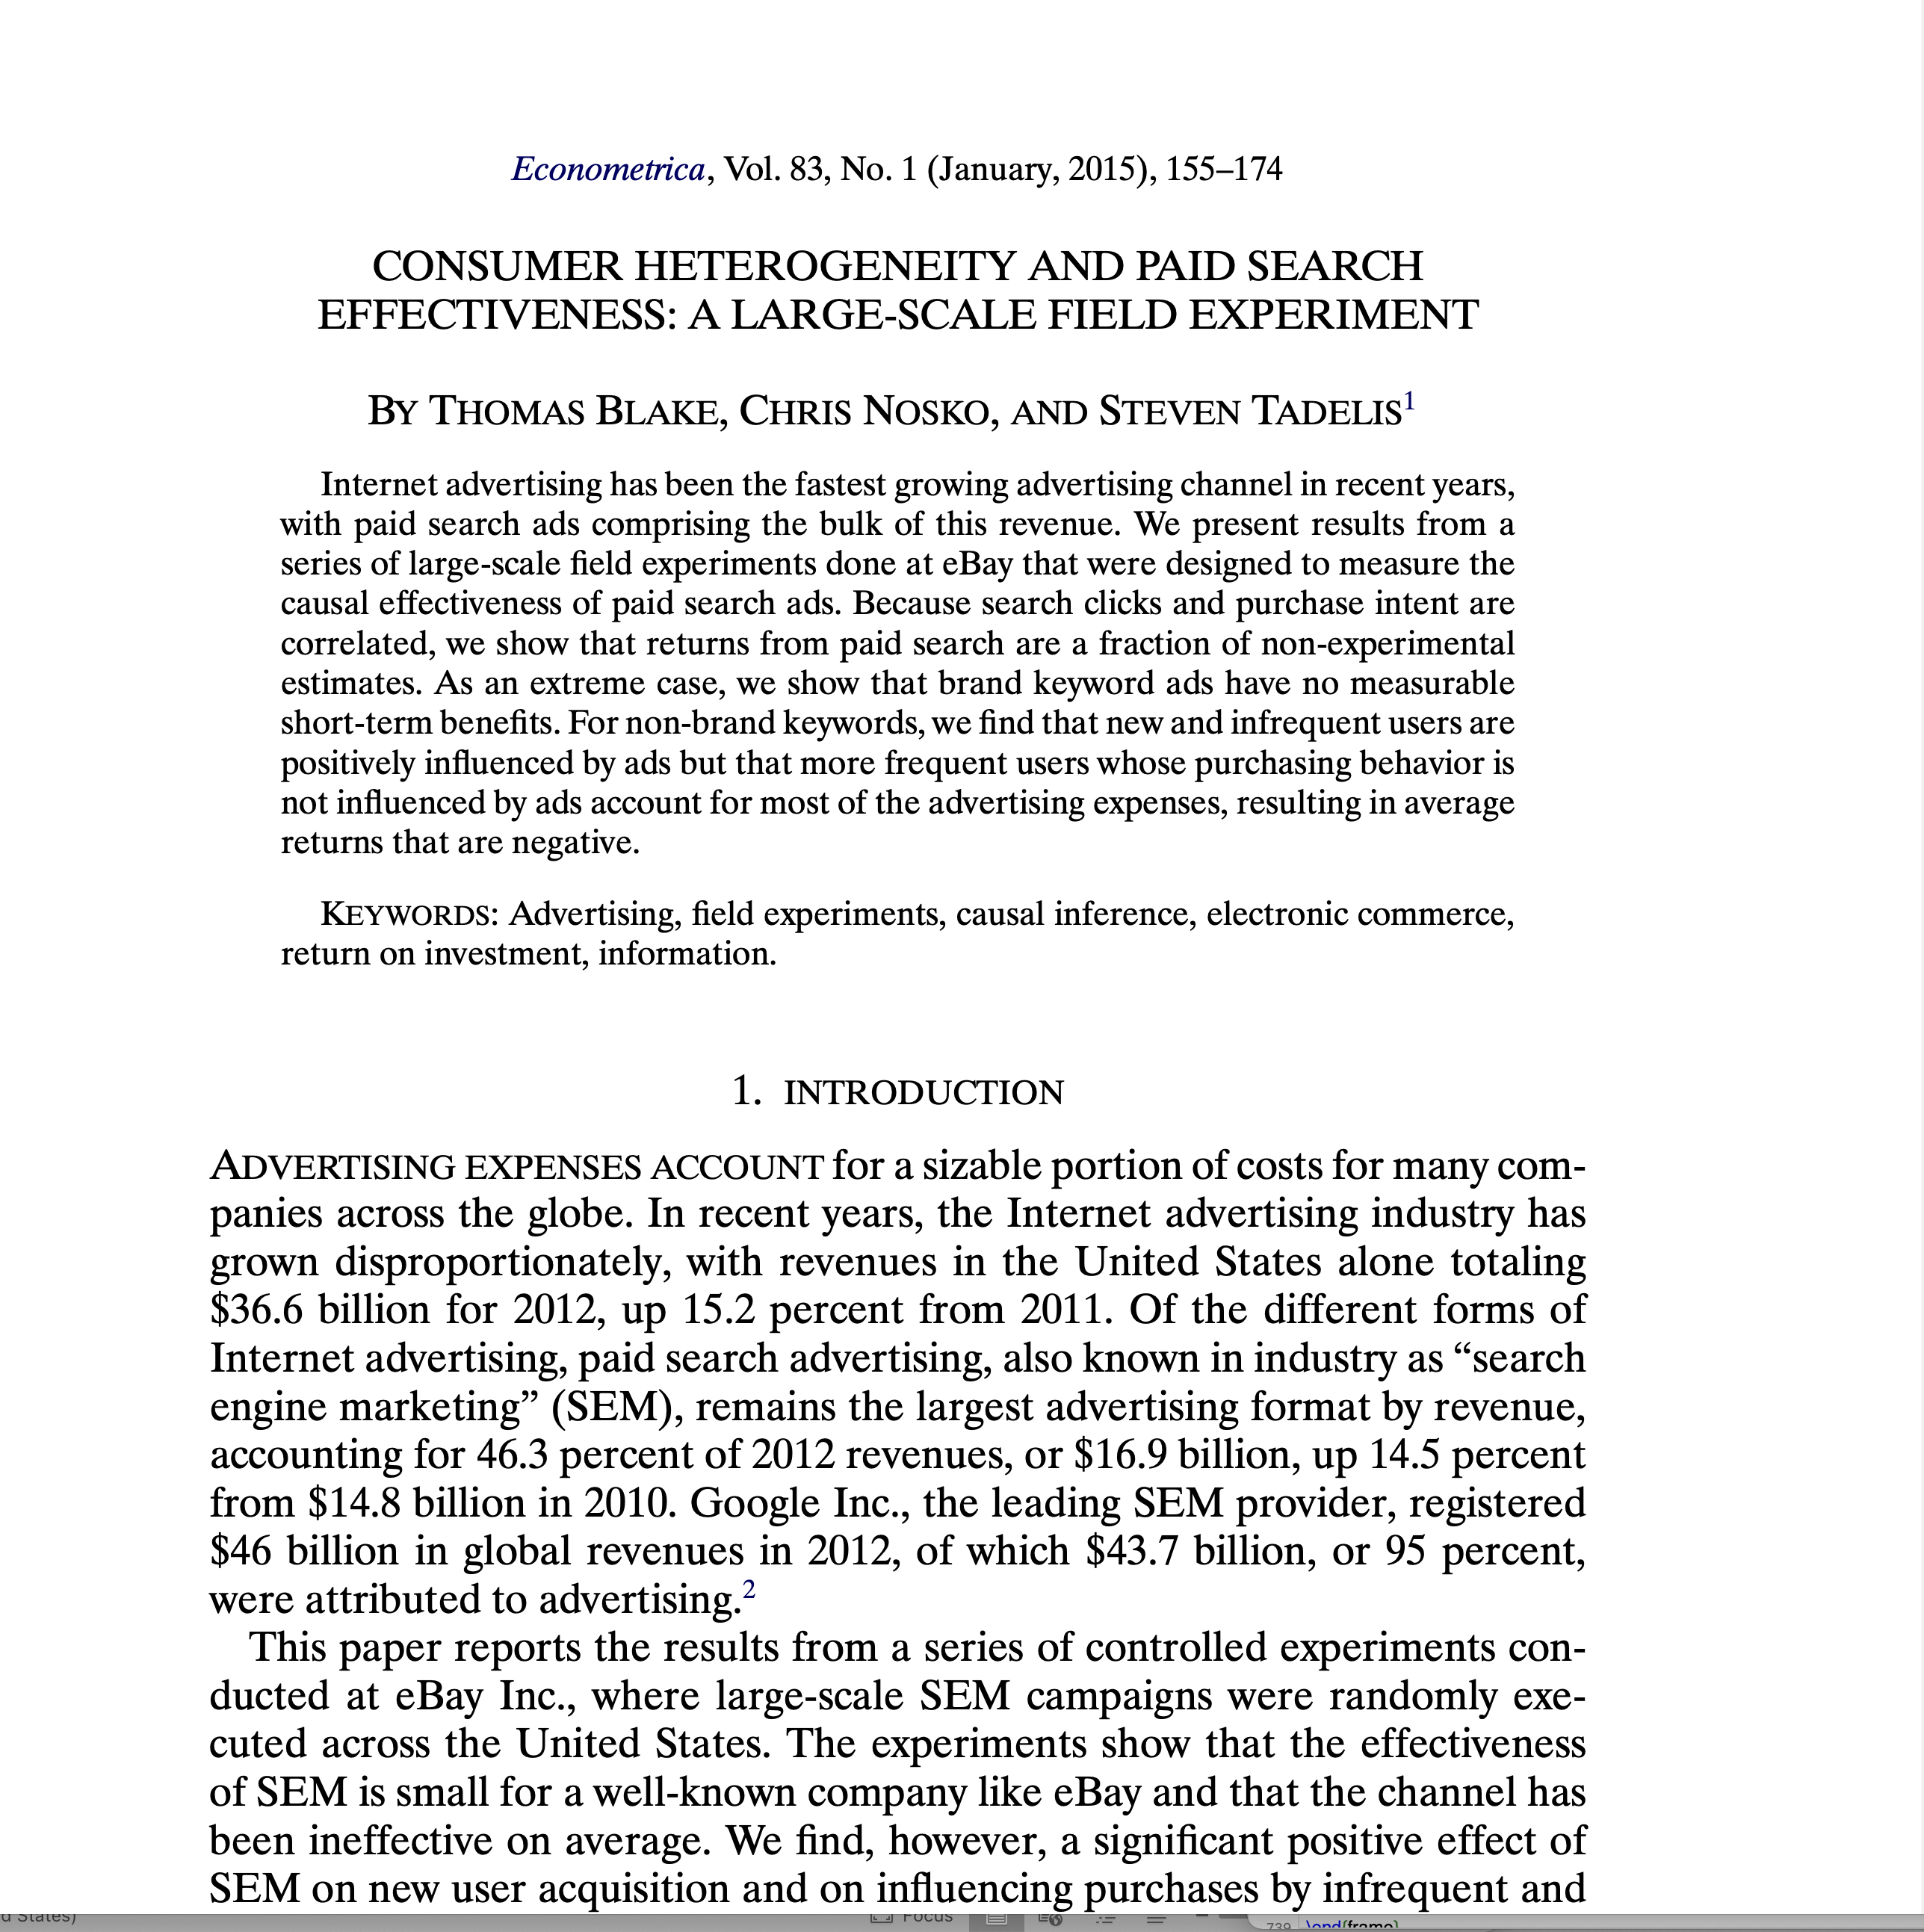
\includegraphics[scale=0.25]{./lecture_includes/econometrica_steve.png}
\end{center}
\end{figure}

\end{frame}

\begin{frame}{Internet advertising facts}

\begin{itemize}
\item In 2012, revenues from Internet advertising was \$36.6 billion and has only grown since
\item Paid search (``search engine marketing'') is the largest format by revenue (46.3\% of 2012 revenues, or \$16.9 billion)
\item Google is leading provider (registered \$46 billion in global revenues in 2012 of which 95\% was attributed to advertising)
\end{itemize}

\end{frame}

\begin{frame}{Selection bias}

\begin{itemize}
\item Treatment was targeted ads at particular people conducting particular types of keyword search
\item Consumers who choose to click on ads are loyal and already informed about products with high likelihood to buy already 
\item Problem is ads are targeting people at the end of their search, so the question is whether they would've found it already (i.e., $E[Y^0|D=1] \neq E[Y^0|D=0]$)
\end{itemize}


\end{frame}



\begin{frame}{Selection bias}

\begin{itemize}
\item Estimated return on investment using OLS  found ROI of over 1600\%
\item Compared this to experimental methods and found ROI of -63\% with a 95\% CI of $[-124\%, -3\%]$, rejecting the hypothesis that the channel yielded short-run positive returns
\item Think back to perfect doctor -- Even without the treatment ($Y^0$), the treated group observationally would've still found a way
\end{itemize}

\end{frame}

\begin{frame}{Natural experiment}

\begin{itemize}
\item Study began with a naturally occurring and somewhat fortuitous  event at eBay
\item eBay halted SEM queries for brand words (i.e., queries that included the term eBay) on Yahoo! and Microsoft but continued to pay for these terms on Google
\item Blake, Nosky and Tadelis (2015) showed almost all of the foregone click traffic and attributed sales were captured by natural search
\item Substitution between paid and unpaid traffic was nearly one to one complete
\end{itemize}

\end{frame}


\begin{frame}

\begin{figure}
\begin{center}
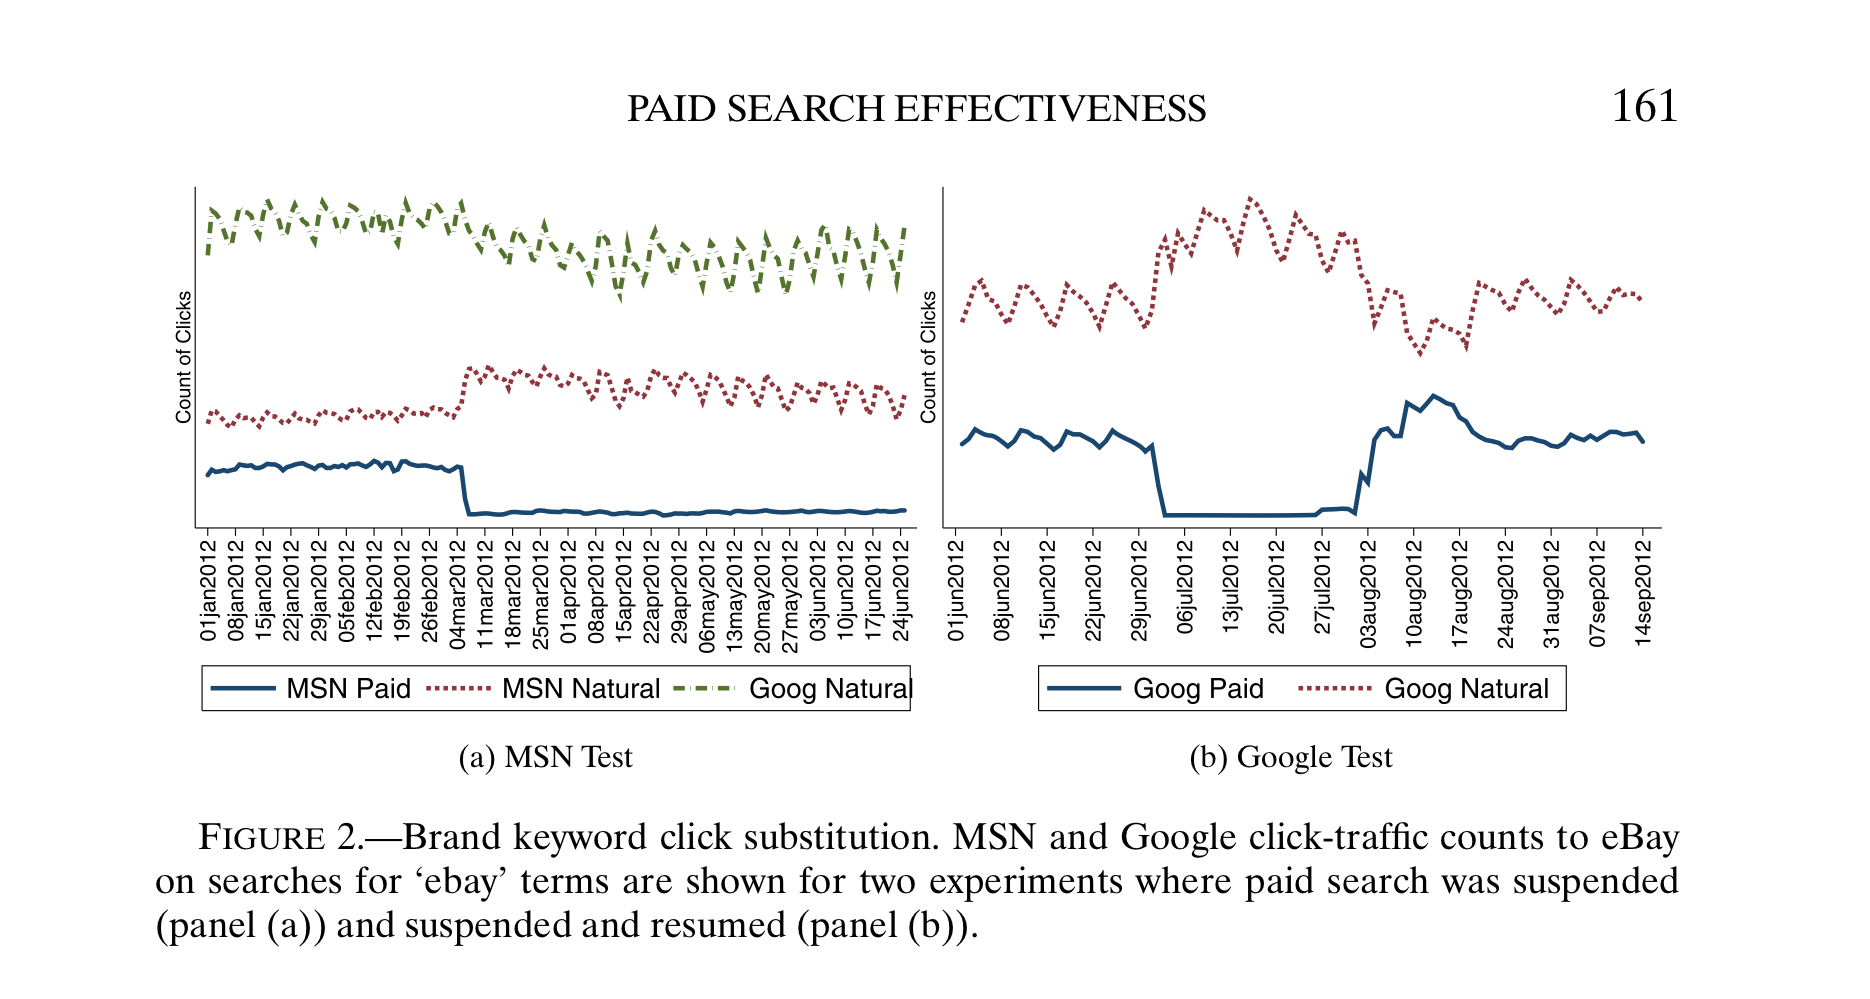
\includegraphics[scale=0.2]{./lecture_includes/tadelis_fig1.png}
\end{center}
\end{figure}

\end{frame}

\begin{frame}{Interpretation of natural experiment}

\begin{quote}
``The evidence strongly supports the intuitive notion that for brand keywords, natural search is close to a perfect substitute for paid search, making brand keyword SEM ineffective for short-term sales.  After all, the users who type the brand keyword in the search query intend to reach the company's website, and most likely will execute on their intent regardless of the appearance of a paid search ad.''
\end{quote}

\end{frame}

\begin{frame}{Selection bias}

Observational data masked causal effect (recall the decomposition of the any non-designed estimation strategy)

\bigskip

\begin{quote}
``Advertising may appear to attract these consumers, when in reality they would have found other channels to visit the company's website.  We overcome this endogeneity challenge with our controlled experiments.''
\end{quote}

\end{frame}




\begin{frame}{RCT}

Natural experiment was valuable, but eBay could run a large scale RCT.

\bigskip


Use this finding of a nearly one-to-one substitution once paid search was dropped to convince eBay to field a large scale RCT discontinuing non-band key words

\bigskip


\end{frame}

\begin{frame}{Design of the experiment}

\begin{itemize}
\item Randomly assigned 30 percent of eBay's US traffic to stop all bidding for all non-brand keywords for 60 days
\item Some random group of users, in other words, were exposed to ads; a control group did not see the ads
\item Used Google's geographic bid feature that can accurately identify geographic market of the user conducting the search
\item Ads were suspended in 30 percent of markets to reduce the scope of the test and minimize the potential cost and impact to the business
\end{itemize}

\end{frame}

\begin{frame}

\begin{figure}
\begin{center}
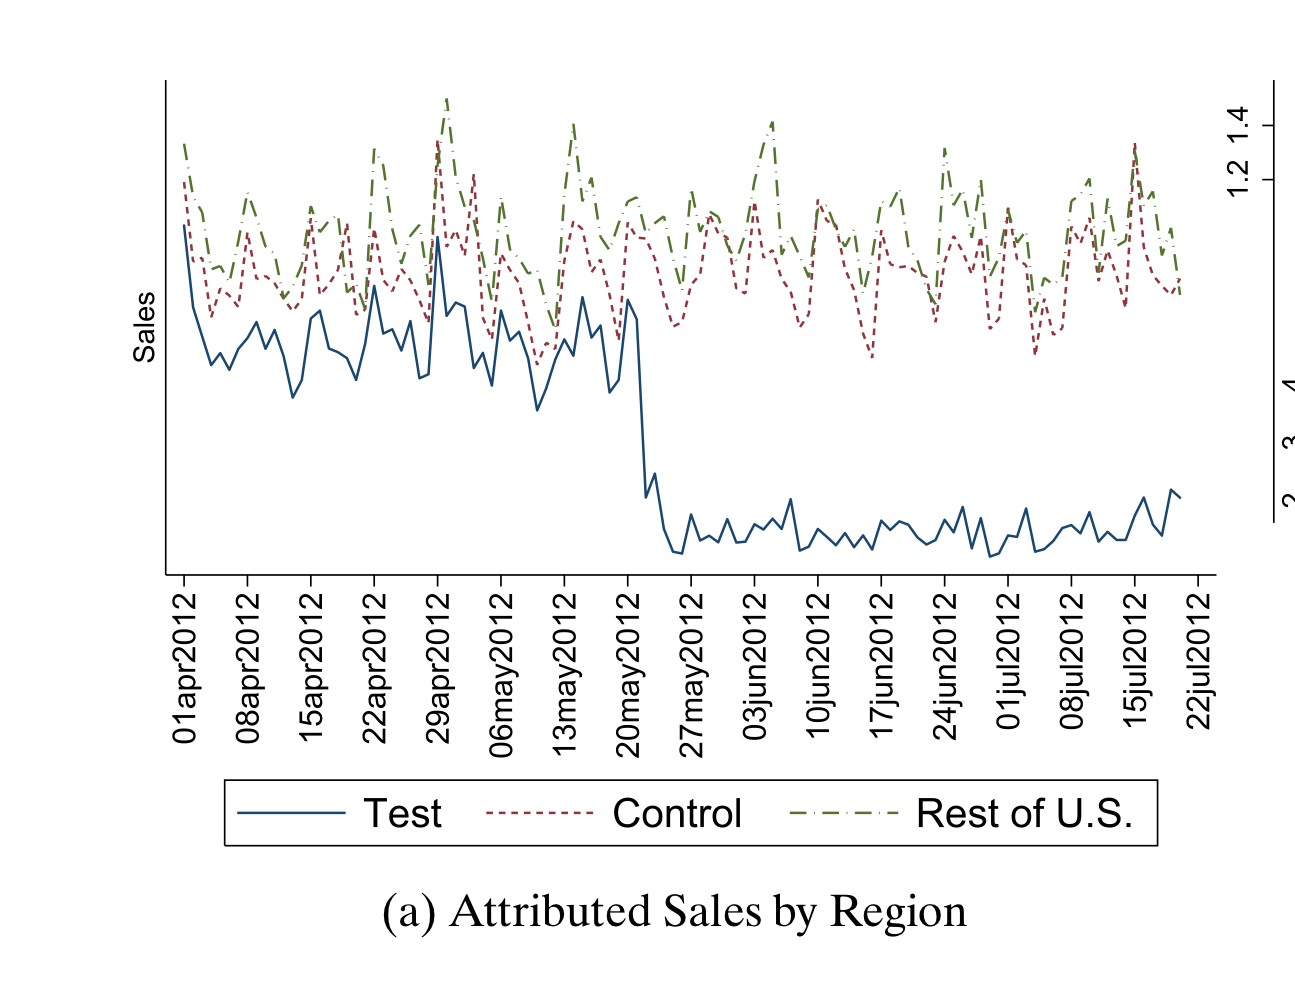
\includegraphics[scale=0.2]{./lecture_includes/tadelis_fig3.png}
\caption{Attributed sales due to clicking on a Google link (treatment group)}
\end{center}
\end{figure}

\end{frame}


\begin{frame}

\begin{figure}
\begin{center}
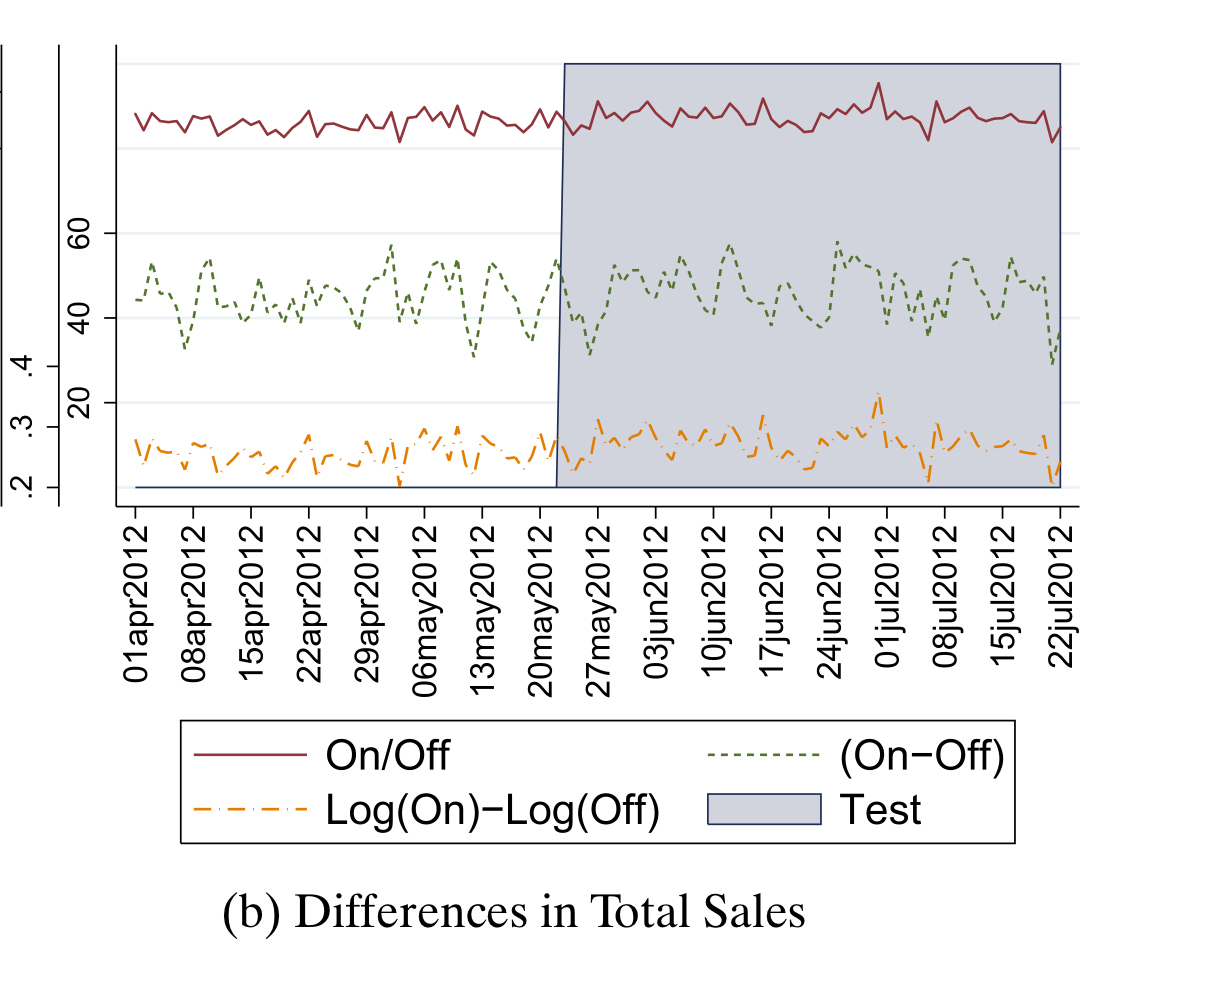
\includegraphics[scale=0.2]{./lecture_includes/tadelis_fig2.png}
\caption{Differences in total sales by market (treatment to control)}
\end{center}
\end{figure}

\end{frame}

\begin{frame}

\begin{figure}
\begin{center}
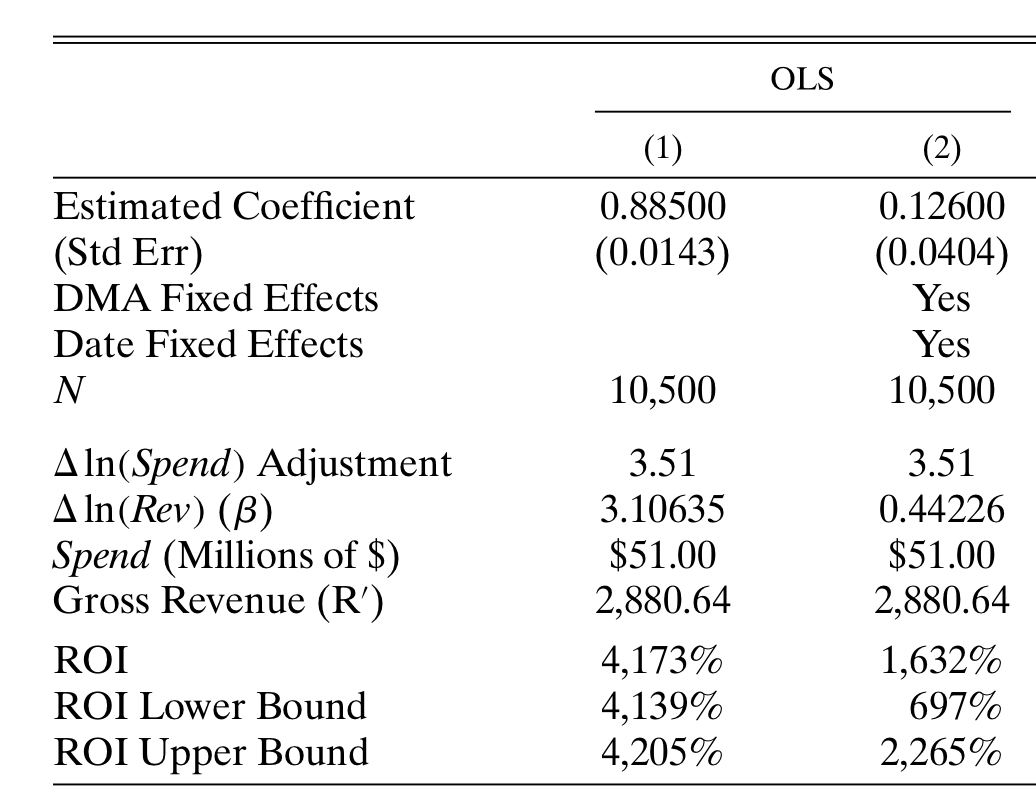
\includegraphics[scale=0.2]{./lecture_includes/tadelis_ols1.png}
\caption{Spending effect on revenue using OLS but not the randomization. Effects are gigantic. }
\end{center}
\end{figure}

\end{frame}

\begin{frame}

\begin{figure}
\begin{center}
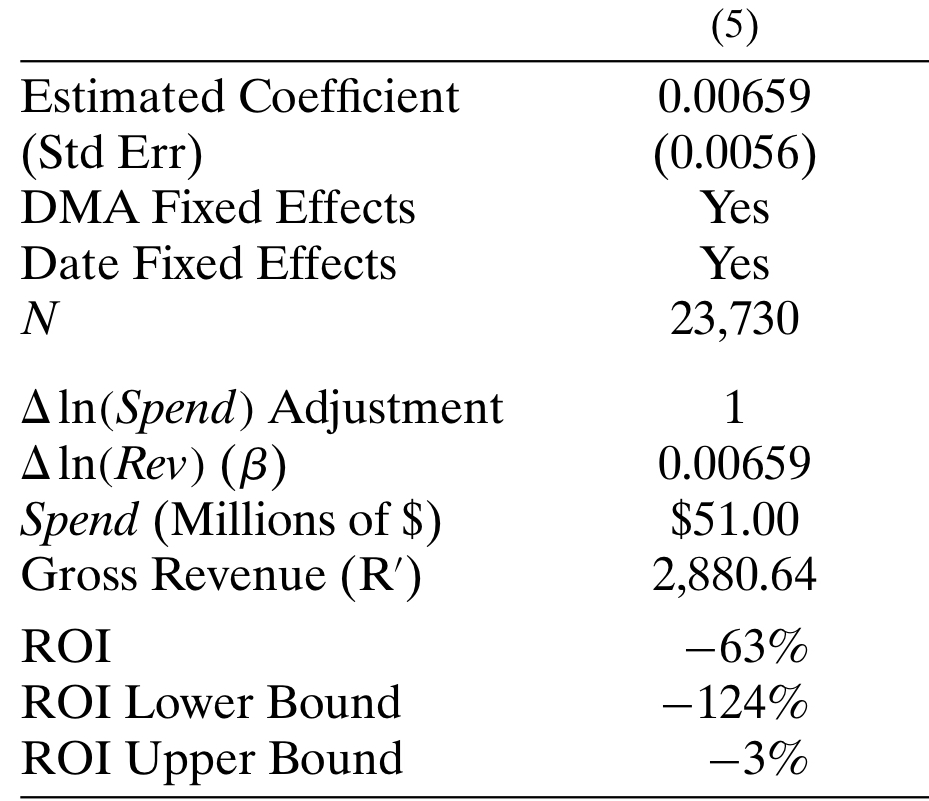
\includegraphics[scale=0.2]{./lecture_includes/tadelis_ols2.png}
\caption{Spending effect on revenue using the randomization. Effects are negative. }
\end{center}
\end{figure}

\end{frame}

\begin{frame}{Heterogenous treatment effects}

\begin{itemize}
\item Recall how the potential outcomes model explicitly models individual treatment effects could be unique and that the perfect doctor showed selection on gains masked treatment effects, perhaps even reversing sign
\item Search advertising in this RCT only worked if the consumer had no idea that the company had the desired product
\item Large firms like eBay with powerful brands will see little benefit from paid search advertising because most consumers already know that they exist, as well as what they have to offer
\end{itemize}

\end{frame}


\begin{frame}

\begin{figure}
\begin{center}
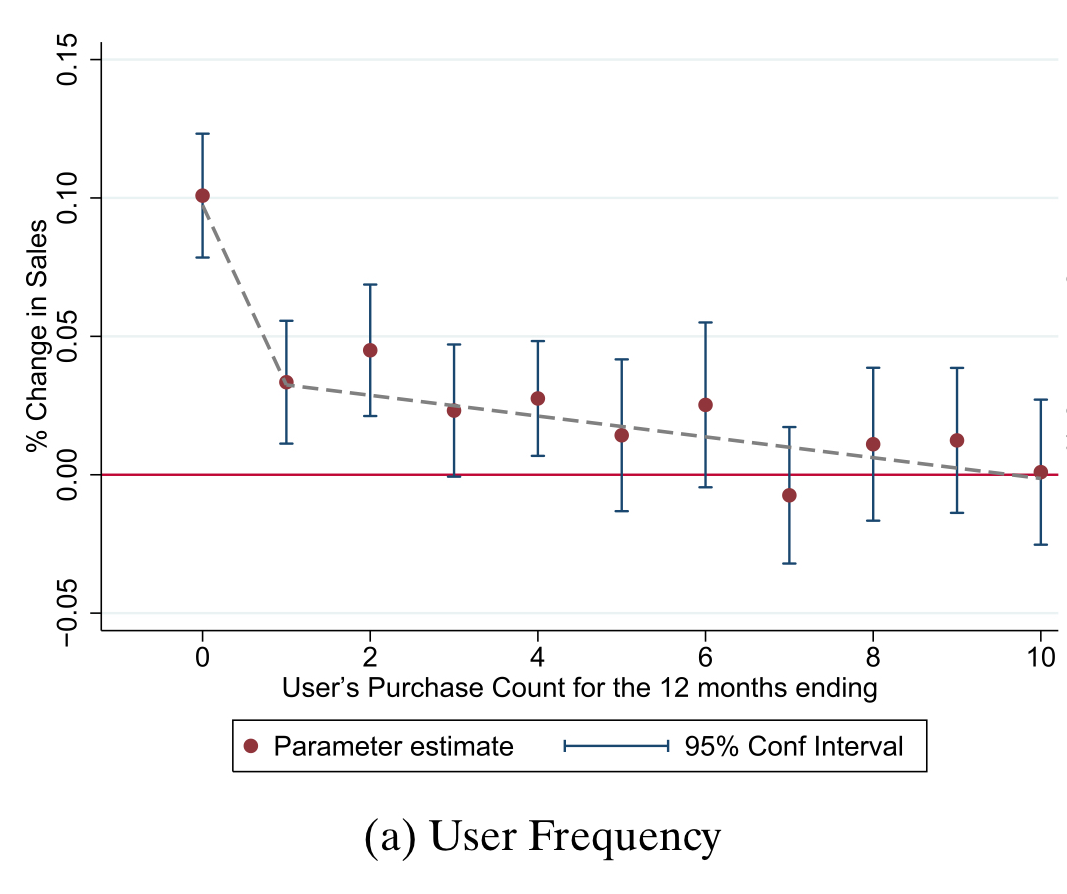
\includegraphics[scale=0.2]{./lecture_includes/tadelis_newuser_fig1.png}
\caption{Effects on new users are positive and large, but not others. }
\end{center}
\end{figure}

\end{frame}

\begin{frame}

\begin{figure}
\begin{center}
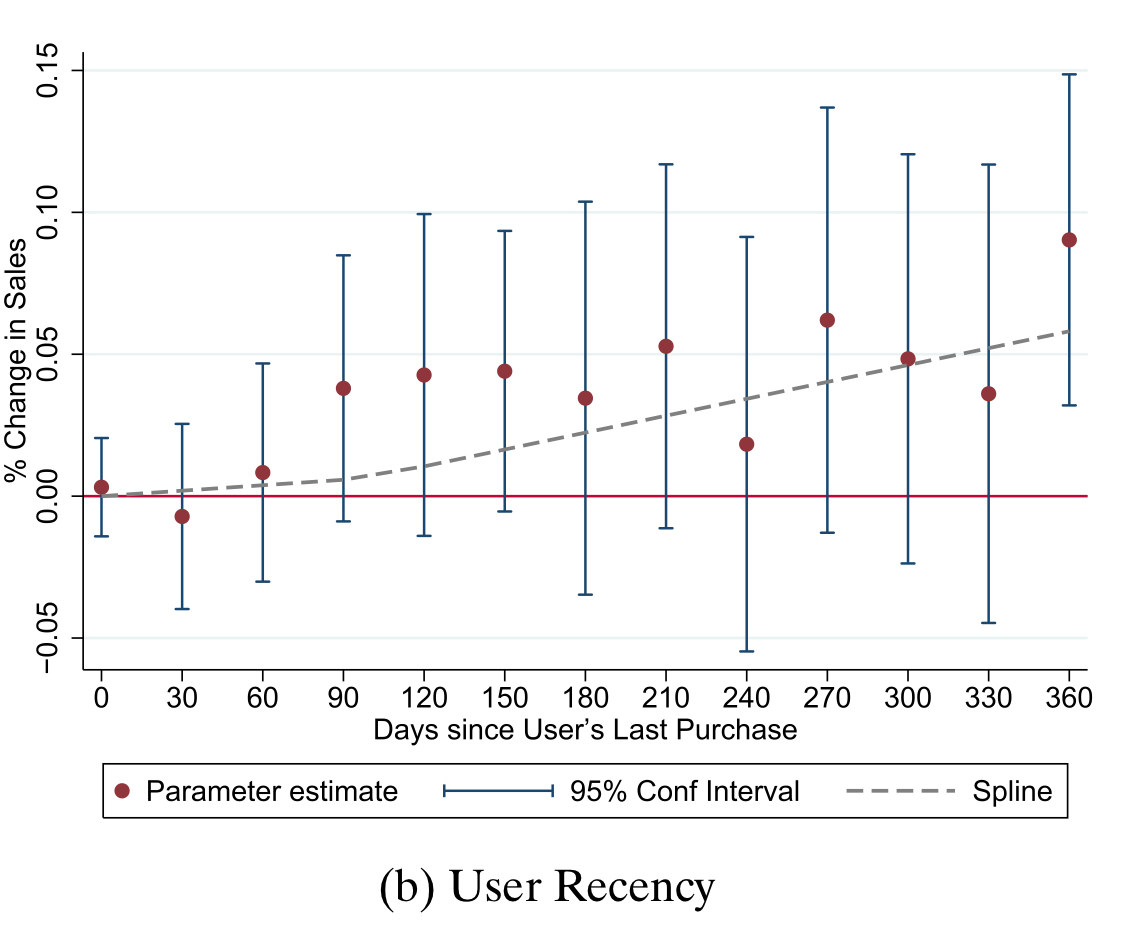
\includegraphics[scale=0.2]{./lecture_includes/tadelis_newuser_fig2.png}
\caption{Effects are largest for ``least active'' customers. }
\end{center}
\end{figure}

\end{frame}


\begin{frame}{Why are causal effects small?}

\begin{itemize}
\item They suggest that the brand query tests found small causal returns because users simply substituted from the paid search clicks to the natural search clicks
\item If that's the case, then it's explicitly a selection bias story $$E[Y^0|D=1] \neq E[Y^0|D=0]$$ where $D$ is being shown the branded advertisement based on search (i.e., they were already going there)
\item They weren't using branded search for information; they were using to \emph{navigate}
\end{itemize}

\end{frame}

\begin{frame}{Self selection based on gains}

\begin{itemize}
\item Potential outcomes is the foundation of the physical experiment because the physical experiment assigns units to treatments \emph{independent} of potential outcomes, $Y^0,Y^1$
\item This is important because outside of the physical experiment, we expect people select those important treatments based on whether, subjectively, they think $Y^1>Y^0$ or $Y^1\leq Y^0$. 
\item Rational actors almost by definition are thought to ``self-select into treatment'' making non-designed comparisons potentially misleading -- sometimes by a little, sometimes by a lot
\end{itemize}

\end{frame}


\begin{frame}{Discussion}

\begin{itemize}
\item What's a correlation that you have heard of or seen that you think is misinterpreted because of selection bias?
\item If you had all the money in the world and complete discretion, what RCT would you run to test it?
\end{itemize}

\end{frame}



\subsection{Example of physical experimentation: HIV status}

\begin{frame}{Demand for Learning HIV Status}


  \begin{itemize}
    \item Rebecca Thornton implemented an RCT in rural Malawi for her job market paper at Harvard in mid-2000s
    \item At the time, it was an article of faith that you could fight the HIV epidemic in Africa by encouraging people to get tested; but Thornton wanted to see if this was true
    \item She randomly assigned cash incentives to people to incentivize learning their HIV status
    \item Also examined whether learning changed sexual behavior.
  \end{itemize}

\end{frame}

\begin{frame}{Experimental design}

  \begin{itemize}
    \item Respondents were offered a free door-to-door HIV test
    \item Treatment is randomized vouchers worth between zero and three dollars
    \item These vouchers were redeemable once they visited a nearby voluntary counseling and testing center (VCT)
    \item Estimates her models using OLS with controls
  \end{itemize}

\end{frame}


\begin{frame}{Why Include Control Variables?}

  To evaluate experimental data, one may want to add additional controls in the multivariate regression model.  So, instead of estimating the SDO, we might estimate:
  \begin{eqnarray*}
    Y_i = \alpha + \delta D_i + \gamma X_i + \eta_i
  \end{eqnarray*}
\end{frame}


\begin{frame}{Why Control Variables?}
  \begin{itemize}
    \item There are 2 main reasons for including additional controls in the regression models:
          \begin{enumerate}
            \item Conditional random assignment.  Sometimes randomization is done \emph{conditional} on some observable (e.g., gender, school, districts)
            \item Exogenous controls increase precision.  Although control variables $X_i$ are uncorrelated with $D_i$, they may have substantial explanatory power for $Y_i$. Including controls thus reduces variance in the residuals which lowers the standard errors of the regression estimates.
          \end{enumerate}
    \item Ongoing work by econometricians is investigating this more carefully
  \end{itemize}
\end{frame}



\begin{frame}[plain]
  \begin{table}[htbp]\centering
    \scriptsize
    \caption{Impact of Monetary Incentives and Distance on Learning HIV Results}
    \label{tab:thornton_main}
    \centering
    \begin{threeparttable}
      \begin{tabular}{l*{5}{c}}
        \toprule
        \multicolumn{1}{l}{\textbf{}}&
        \multicolumn{1}{c}{\textbf{1}}&
        \multicolumn{1}{c}{\textbf{2}}&
        \multicolumn{1}{c}{\textbf{3}}&
        \multicolumn{1}{c}{\textbf{4}}&
        \multicolumn{1}{c}{\textbf{5}}\\
        \midrule
        Any incentive           & 0.431***  & 0.309*** & 0.219***    & 0.220***    & 0.219 ***
        \\
                                & (0.023)   & (0.026)  & (0.029)     & (0.029)     & (0.029)
        \\
        Amount of incentive     &           & 0.091*** & 0.274***    & 0.274***    & 0.273***
        \\
                                &           & (0.012)  & (0.036)     & (0.035)     & (0.036)
        \\
        Amount of incentive$^2$ &           &          & $-0.063$*** & $-0.063$*** & $-0.063$***
        \\
                                &           &          & (0.011)     & (0.011)     & (0.011)
        \\
        HIV                     & $-0.055$* & $-0.052$ & $-0.05$     & $-0.058$*   & $-0.055$*   \\
                                & (0.031)   & (0.032)  & (0.032)     & (0.031)     & (0.031)
        \\
        Distance (km)           &           &          &             & $-0.076$*** &
        \\
                                &           &          &             & (0.027)     &             \\
        Distance$^2$            &           &          &             & 0.010**     &
        \\
                                &           &          &             & (0.005)     &
        \\\midrule
        Controls                & Yes       & Yes      & Yes         & Yes         & Yes
        \\
        Sample size             & 2,812     & 2,812    & 2,812       & 2,812       & 2,812
        \\
        Average attendance      & 0.69      & 0.69     & 0.69        & 0.69        & 0.69
        \\
        \bottomrule
      \end{tabular}
    \end{threeparttable}
  \end{table}

\end{frame}

\begin{frame}[plain]

  \begin{figure}[htb]\centering
    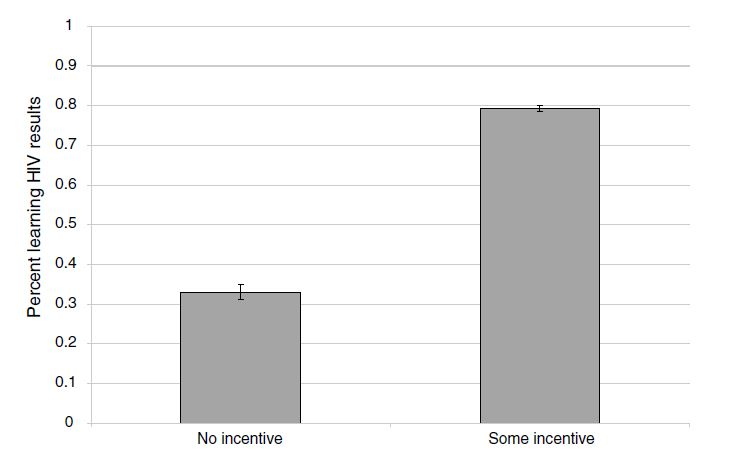
\includegraphics[scale=0.5]{./lecture_includes/FigA.jpg}
    \caption{Visual representation of cash transfers on learning HIV test results.}
    \label{fig:thorntonfig}
  \end{figure}

\end{frame}


\begin{frame}{Results}

  \begin{itemize}
    \item Even small incentives were effective
    \item Any incentive increases learning HIV status by 43\% compared to the control (mean 34\%)
    \item Next she looks at the effect that learning HIV status has on risky sexual behavior
  \end{itemize}

\end{frame}

\begin{frame}[plain]

  \begin{figure}[htb]\centering
    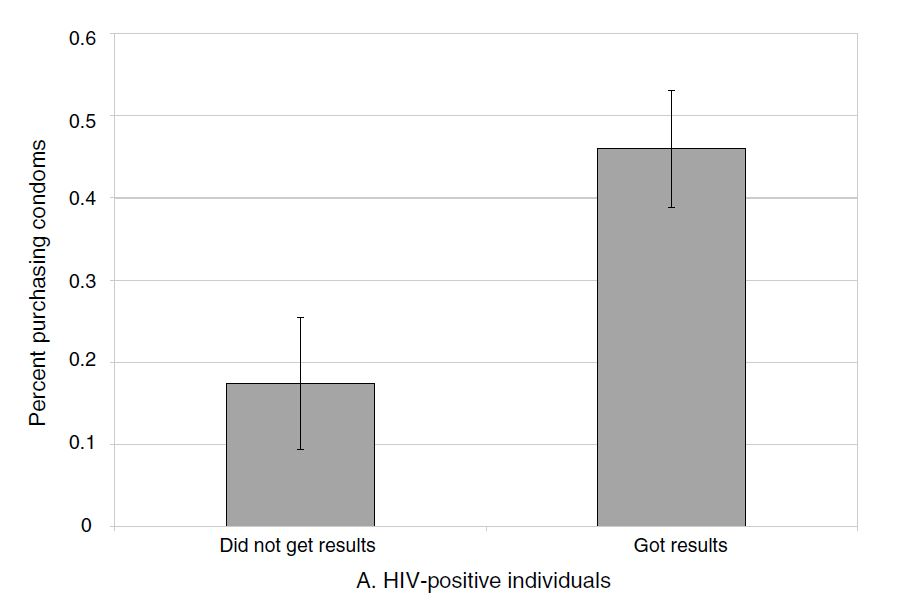
\includegraphics[scale=0.5]{./lecture_includes/FigC.jpg}
    \caption{Visual representation of cash transfers on condom purchases for HIV positive individuals.}
    \label{fig:thorntoncondomfig}
  \end{figure}

\end{frame}

\begin{frame}[plain]

  \begin{table}[htb]\centering
    \scriptsize
    \caption{Reactions to Learning HIV Results among Sexually Active at Baseline}
    \label{tab:thornton_condoms}
    \centering
    \begin{threeparttable}
      \begin{tabular}{l*{5}{c}}
        \toprule
        \multicolumn{1}{l}{\textbf{Dependent variables:}}&
        \multicolumn{2}{c}{\textbf{Bought}}&
        \multicolumn{2}{c}{\textbf{Number of}}\\
        \multicolumn{1}{l}{}&
        \multicolumn{2}{c}{\textbf{condoms}}&
        \multicolumn{2}{c}{\textbf{condoms bought}}\\
        \multicolumn{1}{l}{}&
        \multicolumn{1}{c}{\textbf{OLS}}&
        \multicolumn{1}{c}{\textbf{IV}}&
        \multicolumn{1}{c}{\textbf{OLS}}&
        \multicolumn{1}{c}{\textbf{IV}}\\
        \midrule
        Got results              & $-0.022$   & $-0.069$ & $-0.193$ & $-0.303$
        \\
                                 & (0.025)    & (0.062)  & (0.148)  & (0.285)
        \\
        Got results $\times$ HIV & 0.418***   & 0.248    & 1.778*** & 1.689**
        \\
                                 & (0.143)    & (0.169)  & (0.564)  & (0.784)  \\
        HIV                      & $-0.175$** & $-0.073$ & $-0.873$ & $-0.831$
        \\
                                 & (0.085)    & (0.123)  & (0.275)  & (0.375)  \\\midrule
        Controls                 & Yes        & Yes      & Yes      & Yes
        \\
        Sample size              & 1,008      & 1,008    & 1,008    & 1,008    \\
        Mean                     & 0.26       & 0.26     & 0.95     & 0.95     \\
        \bottomrule
      \end{tabular}
    \end{threeparttable}
  \end{table}

\end{frame}

\begin{frame}{Results}

  \begin{itemize}
    \item For those who were HIV$+$ and got their test results, 42\% more likely to buy condoms (but shrinks and becomes insignificant at conventional levels with IV).
    \item Number of condoms bought -- very small. HIV$+$ respondents who learned their status bought 2 more condoms
  \end{itemize}

\end{frame}

\begin{frame}{Discussion}

  \begin{itemize}
    \item What's in your field a causal question you find interesting that you wish you could answer?
    \item Describe the way you would conduct the RCT by explaining the following:
          \begin{itemize}
            \item What's the treatment?  Express it as a binary variable.
            \item How will you assign this so that SUTVA holds and independence is achieved?
            \item What is the outcome you are interested in?
          \end{itemize}
    \item Describe the steps you would take to do this if you had all the money in the world
  \end{itemize}

\end{frame}

\section{Randomization inference}

\subsection{Lady tasting tea}

\begin{frame}{Randomization inference and causal inference}

\begin{itemize}
\item ``In randomization-based inference, uncertainty in estimates arises naturally from the random assignment of the treatments, rather than from hypothesized sampling from a large population.'' (Athey and Imbens 2017)

\item Athey and Imbens is part of growing trend of economists using randomization-based methods for doing causal inference

\item Unclear (to me) why we are hearing more and more about randomization inference, but we are. 

\item Could be due to improved computational power and/or the availability of large data instead of samples?

\end{itemize}


\end{frame}




\begin{frame}{Lady tasting tea experiment}

	\begin{itemize}
	\item Ronald Aylmer Fisher (1890-1962)
		\begin{itemize}
		\item Two classic books on statistics: \emph{Statistical Methods for Research Workers} (1925) and \emph{The Design of Experiments} (1935), as well as a famous work in genetics, \emph{The Genetical Theory of Natural Science}
		\item Developed many fundamental notions of modern statistics including the theory of randomized experimental design.
		\end{itemize}

	\end{itemize}
	
\end{frame}


\begin{frame}{Lady tasting tea}

\begin{itemize}
	\item Muriel Bristol (1888-1950)
		\begin{itemize}
		\item A PhD scientist back in the days when women weren't PhD scientists
		\item Worked with Fisher at the Rothamsted Experiment Station (which she established) in 1919 
		\item During afternoon tea, Muriel claimed she could tell from taste whether the milk was added to the cup before or after the tea
		\item Scientists were incredulous, but Fisher was inspired by her strong claim
		\item He devised a way to test her claim which she passed using randomization inference
		\end{itemize}
\end{itemize}

\end{frame}

\begin{frame}{Description of the tea-tasting experiment}

	\begin{itemize}
	\item Original claim: Given a cup of tea with milk, Bristol claims she can discriminate the order in which the milk and tea were added to the cup
	\item Experiment: To test her claim, Fisher prepares 8 cups of tea -- 4 \textbf{milk then tea} and 4 \textbf{tea then milk} -- and presents each cup to Bristol for a taste test
	\item Question: How many cups must Bristol correctly identify to convince us of her unusual ability to identify the order in which the milk was poured?
	\item Fisher's sharp null: Assume she can't discriminate.  Then what's the likelihood that random chance was responsible for her answers?
	\end{itemize}
\end{frame}

\begin{frame}{Choosing subsets}
	
	\begin{itemize}
	\item The lady performs the experiment by selecting $4$ cups, say, the ones she claims to have had the tea poured first.
	 $${n \choose k} = \frac{n!}{k!(n-k)!}$$
	\item ``8 choose 4'' -- $ 8 \choose 4 $ -- ways to choose 4 cups out of 8
		
		\begin{itemize}
		\item Numerator is $8\times{7}\times{6}\times{5}=1,680$ ways to choose a first cup, a second cup, a third cup, and a fourth cup, in order.
		\item Denominator is $4\times{3}\times{2}\times{1}=24$ ways to order $4$ cups.
		\end{itemize}
	\end{itemize}
\end{frame}


\begin{frame}{Choosing subsets}

\begin{itemize}
	\item There are $70$ ways to choose $4$ cups out of $8$, and therefore a 1.4\% probability of producing the correct answer by chance
		\begin{eqnarray*}
		\frac{24}{1680}=1/70=0.014.
		\end{eqnarray*}
	\item For example, the probability that she would correctly identify all $4$ cups is $\frac{1}{70}$ 
\end{itemize}

\end{frame}


%\begin{frame}[plain]

%	\begin{center}
%	\textbf{Choosing $3$}
%	\end{center}
	
%	\begin{itemize}
%	\item To get exactly $3$ right, and, hence, $1$ wrong, she would have to choose $3$ from the $4$ correct ones.
%		\begin{enumerate}
%		\item She can do this by $4\times{3}\times{2}=24$ with order.
%		\item Since $3$ cups can be ordered in $3\times{2}=6$ ways, there are $4$ ways for her to choose the $3$ correctly.
%		\end{enumerate}
%	\item Since she can now choose the $1$ incorrect cup $4$ ways, there are a total of $4\times{4}=16$ ways for her to choose exactly $3$ right and $1$ wrong.
%	\item Hence the probability that she chooses exactly 3 correctly is $\frac{16}{70}=0.23$.
%	\end{itemize}
%\end{frame}

\begin{frame}{Statistical significance}
	
	\begin{itemize}
	\item Suppose the lady correctly identifies all 4 cups.  Then \dots
		\begin{enumerate}
		\item Either she has no ability, and has chosen the correct 4 cups purely by chance, or
		\item She has the discriminatory ability she claims.
		\end{enumerate}
	\item Since choosing correctly is highly unlikely in the first case (one chance in $70$), the second seems plausible.
	\item Bristol actually got all four correct
	\item I wonder if seeing this, any of the scientists present changed their mind
	\end{itemize}
\end{frame}

\subsection{Fisher's sharp null}

\begin{frame}{Null hypothesis}
	
	\begin{itemize}
	\item In this example, the null hypothesis is the hypothesis that the lady has no special ability to discriminate between the cups of tea.
	\item We can never prove the null hypothesis, but the data may provide evidence to reject it.
	\item In most situations, rejecting the null hypothesis is what we hope to do.

	\end{itemize}
\end{frame}



\begin{frame}{Null hypothesis of no effect}

\begin{itemize}
\item Randomization inference allows us to make probability calculations revealing whether the treatment assignment was ``unusual''
\item Fisher's sharp null is when entertain the possibility that no unit has a treatment effect
\item This allows us to make ``exact'' p-values which do not depend on large sample approximations
\item It also means the inference is not dependent on any particular distribution (e.g., Gaussian); sometimes called nonparametric
\end{itemize}

\end{frame}




\begin{frame}{Sidebar: bootstrapping is different}

\begin{itemize}
\item Sometimes people confuse randomization inference with bootstrapping
\item Bootstrapping randomly draws a percent of the total observations for estimation; ``uncertainty over the sample''
\item Randomization inference randomly reassigns the treatment;  ``uncertainty over treatment assignment''
\end{itemize}(Thanks to Jason Kerwin for helping frame the two against each other)

\end{frame}


\begin{frame}{6-step guide to randomization inference}

\begin{enumerate}
\item Choose a sharp null hypothesis (e.g., no treatment effects)
\item Calculate a test statistic ($T$ is a scalar based on $D$ and $Y$)
\item Then pick a randomized treatment vector $\tilde{D_1}$
\item Calculate the test statistic associated with $(\tilde{D},Y)$
\item Repeat steps 3 and 4 for all possible combinations to get $\tilde{T} = \{\tilde{T}_1, \dots , \tilde{T}_K \}$
\item Calculate exact p-value as $p=\frac{1}{K} \sum_{k=1}^K I(\tilde{T}_k \geq T)$
\end{enumerate}
\end{frame}


\begin{frame}{Pretend experiment}

\begin{table}[htbp]\centering
\begin{center}
\caption{Pretend DBT intervention for some homeless population}
\begin{threeparttable}
\begin{tabular}{lcccc}
\toprule
\multicolumn{1}{l}{Name}&
\multicolumn{1}{c}{D}&
\multicolumn{1}{c}{Y}&
\multicolumn{1}{c}{Y$^0$}&
\multicolumn{1}{c}{Y$^1$}\\
\midrule
Andy		& 1 & 10  & . & 10 \\
Ben		& 1 & 5    & . & 5 \\
Chad	& 1 & 16  & . & 16 \\	
Daniel	& 1 &  3   & . & 3 \\
Edith		& 0 & 5    & 5 & . \\
Frank	& 0 & 7    & 7&.  \\
George	& 0 & 8    & 8 & . \\
Hank		& 0 & 10  & 10 & . \\
\bottomrule
\end{tabular}
\end{threeparttable}
\end{center}
\end{table}

For concreteness, assume a program where we pay homeless people \$15 to take dialectical behavioral therapy (DBT). Outcomes are some measure of mental health 0-20 with higher scores being improvements in mental health symptoms. 
	
\end{frame}



\begin{frame}{Step 1: Sharp null of no effect}

\begin{block}{Fisher's Sharp Null Hypothesis}
$H_0: \delta_i = Y_i^1 - Y_i^0 = 0 \text{ } \forall i$
\end{block}

\begin{itemize}
\item Assuming no effect means any test statistic is due to chance
\item Neyman and Fisher test statistics were different -- Fisher was exact, Neyman was not
\item Neyman's null was no average treatment effect (ATE=0). If you have a treatment effect of 5 and I have a treatment effect of -5, our ATE is zero. This is not the sharp null even though it also implies a zero ATE

\end{itemize}

\end{frame}


\begin{frame}{More sharp null}

\begin{itemize}
\item Since under the Fisher sharp null $\delta_i=0$, it means each unit's potential outcomes under both states of the world are the same
\item We therefore know each unit's missing counterfactual
\item The randomization we will perform will cycle through all treatment assignments under a null well treatment assignment doesn't matter because all treatment assignments are associated with a null of zero unit treatment effects
\item We are looking for evidence \emph{against} the null 
\end{itemize}

\end{frame}




\begin{frame}{Step 1: Fisher's sharp null and missing potential outcomes}

\begin{table}[htbp]\centering
\begin{center}
\caption{Missing potential outcomes are no longer missing}
\begin{threeparttable}
\begin{tabular}{lcccc}
\toprule
\multicolumn{1}{l}{Name}&
\multicolumn{1}{c}{D}&
\multicolumn{1}{c}{Y}&
\multicolumn{1}{c}{Y$^0$}&
\multicolumn{1}{c}{Y$^1$}\\
\midrule
Andy		& 1 & 10  & \textbf{10} & 10 \\
Ben		& 1 & 5    & \textbf{5} & 5 \\
Chad	& 1 & 16  & \textbf{16} & 16 \\	
Daniel	& 1 &  3   & \textbf{3} & 3 \\
Edith		& 0 & 5    & 5 & \textbf{5} \\
Frank	& 0 & 7    & 7& \textbf{7}  \\
George	& 0 & 8    & 8 & \textbf{8} \\
Hank		& 0 & 10  & 10 & \textbf{10} \\
\bottomrule
\end{tabular}
\end{threeparttable}
\end{center}
\end{table}

Fisher sharp null allows us to \textbf{fill in} the missing counterfactuals bc under the null there's zero treatment effect at the unit level.
	
\end{frame}

\begin{frame}{Step 2: Choosing a test statistic}

\begin{block}{Test Statistic}
A test statistic $T(D,Y)$ is a scalar quantity calculated from the treatment assignments  $D$ and the observed outcomes $Y$ 
\end{block}

\begin{itemize}
\item By scalar, I just mean it's a number (vs. a function) measuring some relationship between $D$ and $Y$
\item Ultimately there are many tests to choose from; I'll review a few later
\item If you want a test statistic with high statistical power, you need large values when the null is false, and small values when the null is true (i.e., \emph{extreme})
\end{itemize}

\end{frame}

\begin{frame}{Simple difference in means}

\begin{itemize}
\item Consider the absolute SDO from earlier $$ \delta_{SDO} = \bigg | \frac{1}{N_T} \sum_{i=1}^N D_iY_i - \frac{1}{N_C} \sum_{i=1}^N (1-D_i)Y_i \bigg |$$
\item Larger values of $\delta_{SDO}$ are evidence \emph{against} the sharp null
\item Good estimator for constant, additive treatment effects and relatively few outliers in the potential outcomes
\end{itemize}

\end{frame}

\begin{frame}{Step 2: Calculate test statistic, $T(D,Y)$}

\begin{table}[htbp]\centering
\begin{center}
\caption{Calculate $T$ using $D$ and $Y$}
\begin{threeparttable}
\begin{tabular}{lccccc}
\toprule
\multicolumn{1}{l}{Name}&
\multicolumn{1}{c}{D}&
\multicolumn{1}{c}{Y}&
\multicolumn{1}{c}{Y$^0$}&
\multicolumn{1}{c}{Y$^1$}&
\multicolumn{1}{c}{$\delta_i$}\\
\midrule
Andy		& \textbf{1} & \textbf{10}  & {10} & {10} & 0\\
Ben		& \textbf{1} & \textbf{5}    & {5} & {5} & 0 \\
Chad	& \textbf{1} & \textbf{16}  & {16} & {16} & 0 \\	
Daniel	& \textbf{1} &  \textbf{3}   & {3} & {3} & 0 \\
Edith		& \textbf{0} & \textbf{5}    & {5} & {5} & 0 \\
Frank	& \textbf{0} & \textbf{7}    & {7} & {7} & 0  \\
George	& \textbf{0} &\textbf {8}    & {8} & {8} & 0 \\
Hank		& \textbf{0} & \textbf{10}  & {10} & {10} & 0 \\
\bottomrule
\end{tabular}
\end{threeparttable}
\end{center}
\end{table}

We'll start with this simple the simple difference in means test statistic, $T(D,Y)$: $\delta_{SDO} = 34/4 - 30/4 = 1$	
\end{frame}



\begin{frame}{Steps 3-5: Null randomization distribution}

\begin{itemize}
\item Randomization steps reassign treatment assignment for every combination, calculating test statistics each time, to obtain the entire distribution of counterfactual test statistics
\item The key insight of randomization inference is that under Fisher's sharp null, the treatment assignment shouldn't matter
\item Ask yourself: 
	\begin{itemize}
	\item if there is no unit level treatment effect, can you picture a distribution of counterfactual test statistics?
	\item and if there is no unit level treatment effect, what must average counterfactual test statistics equal?
	\end{itemize}
\end{itemize}

\end{frame}

\begin{frame}{Step 6: Calculate ``exact'' p-values}

\begin{itemize}
\item Question: how often would we get a test statistic as big or bigger as our ``real'' one if Fisher's sharp null was true?
\item This can be calculated ``easily'' (sometimes) once we have the randomization distribution from steps 3-5
	\begin{itemize}
	\item The number of test statistics ($t(D,Y)$) bigger than the observed divided by total number of randomizations $$Pr(T(D,Y) \geq T(\tilde{D},Y | \delta = 0)) = \frac{ \sum_{D \in \Omega} I(T(D,Y) \leq T(\tilde{D},Y)}{K}$$
	\end{itemize}
\end{itemize}
\end{frame}


%\begin{frame}[plain]

%\begin{center}
%\textbf{Simulation}
%\end{center}

%Download the file \texttt{combinations.do} and you can do this yourself for this dataset of eight people.  It will do exact combinations. 

%\end{frame}


\begin{frame}{First permutation (holding $N_T$ fixed)}

\begin{table}[htbp]\centering
\begin{center}
\begin{threeparttable}
\begin{tabular}{lcccc}
\toprule
\multicolumn{1}{l}{Name}&
\multicolumn{1}{c}{$\tilde{D_2}$}&
\multicolumn{1}{c}{Y}&
\multicolumn{1}{c}{Y$^0$}&
\multicolumn{1}{c}{Y$^1$}\\
Andy		& 1 & \textcolor{blue}{10}  & {10} & 10 \\
Ben		& 0 & \textcolor{red}{5}    & {5} & 5 \\
Chad	& 1 & \textcolor{blue}{16}  & {16} & 16 \\	
Daniel	& 1 &  \textcolor{blue}{3}   & {3} & 3 \\
Edith		& 0 & \textcolor{red}{5}    & 5 & {5} \\
Frank	& 1 & \textcolor{blue}{7}    & 7& {7}  \\
George	& 0 & \textcolor{red}{8}    & 8 & {8} \\
Hank		& 0 & \textcolor{red}{10}  & 10 & {10} \\
\bottomrule
\end{tabular}
\end{threeparttable}
\end{center}
\end{table}

$$\tilde{T}_1 =  | \textcolor{blue}{36/4} - \textcolor{red}{28/4}  | = \textcolor{blue}{9} - \textcolor{red}{7} = 2$$
	
\end{frame}

\begin{frame}{Second permutation (again holding $N_T$ fixed)}

\begin{table}[htbp]\centering
\begin{center}
\begin{threeparttable}
\begin{tabular}{lcccc}
\toprule
\multicolumn{1}{l}{Name}&
\multicolumn{1}{c}{$\tilde{D_3}$}&
\multicolumn{1}{c}{Y}&
\multicolumn{1}{c}{Y$^0$}&
\multicolumn{1}{c}{Y$^1$}\\
Andy		& 1 & \textcolor{blue}{10}  & {10} & 10 \\
Ben		& 0 & \textcolor{red}{5}    & {5} & 5 \\
Chad	& 1 & \textcolor{blue}{16}  & {16} & 16 \\	
Daniel	& 1 &  \textcolor{blue}{3}   & {3} & 3 \\
Edith		& 0 & \textcolor{red}{5}    & 5 & {5} \\
Frank	& 0 & \textcolor{red}{7}    & 7& {7}  \\
George	& 1 & \textcolor{blue}{8}    & 8 & {8} \\
Hank		& 0 & \textcolor{red}{10}  & 10 & {10} \\
\bottomrule
\end{tabular}
\end{threeparttable}
\end{center}
\end{table}

$$T_{rank} =  | \textcolor{blue}{36/4} - \textcolor{red}{27/4}  | = \textcolor{blue}{9} - \textcolor{red}{6.75} = 2.25$$
	
\end{frame}

\begin{frame}{Sidebar: Should it be 4 treatment groups each time?}

\begin{itemize}
\item In this experiment, I've been using the same $N_T$ \emph{under the assumption} that $N_T$ had been fixed when the experiment was drawn.
\item But if the original treatment assignment had been generated by something like a Bernoulli distribution (e.g., coin flips over every unit), then you should be doing a complete permutation that is also random in this way
\item This means that for 8 units, sometimes you'd have 1 treated, or even 8
\item Correct inference requires you know the original data generating process
\end{itemize}

\end{frame}

\begin{frame}{Randomization distribution}

\begin{table}[htbp]\centering
\begin{center}
\begin{threeparttable}
\begin{tabular}{lccccccccc}
\toprule
\multicolumn{1}{l}{Assignment}&
\multicolumn{1}{c}{$D_1$}&
\multicolumn{1}{c}{$D_2$}&
\multicolumn{1}{c}{$D_3$}&
\multicolumn{1}{c}{$D_4$}&
\multicolumn{1}{c}{$D_5$}&
\multicolumn{1}{c}{$D_6$}&
\multicolumn{1}{c}{$D_7$}&
\multicolumn{1}{c}{$D_8$}&
\multicolumn{1}{c}{$|T_i|$}\\
\midrule
True $D$ & 1 & 1 & 1 & 1 & 0 & 0 & 0 & 0 & 1 \\
$\tilde{D_2}$ & 1 & 0 & 1 & 1 & 0 & 1 & 0 & 0 & 2 \\
$\tilde{D_3}$ & 1 & 0 & 1 & 1 & 0 & 0 & 1 & 0 & 2.25 \\
\dots \\
\bottomrule
\end{tabular}
\end{threeparttable}
\end{center}
\end{table}

\end{frame}

\subsection{Alternative test statistics}

\begin{frame}{Step 2: Other test statistics}

\begin{itemize}
\item The simple difference in means is fine when effects are additive, and there are few outliers in the data
\item But outliers create more variation in the randomization distribution
\item A good test statistic is the one that best fits your data.  
\item Some test statistics will have weird properties in the randomization as we'll see in synthetic control.
\item What are some alternative test statistics?
\end{itemize}

\end{frame}

\begin{frame}{Transformations}

\begin{itemize}
\item What if there was a constant multiplicative effect: $Y_i^1 / Y_i^0 = C$?
\item Difference in means will have low power to detect this alternative hypothesis
\item So we transform the observed outcome using the natural log:

$$T_{log} = \bigg | \frac{1}{N_T} \sum_{i=1}^N D_i ln(Y_i) - \frac{1}{N_C} \sum_{i=1}^N (1-D_i) ln(Y_i) \bigg |$$
\item This is useful for skewed distributions of outcomes

\end{itemize}

\end{frame}

\begin{frame}{Difference in medians/quantiles}

\begin{itemize}
\item We can protect against outliers using other test statistics such as the difference in quantiles
\item Difference in medians:$$T_{median} = | median(Y_T) - median(Y_C)|$$
\item We could also estimate the difference in quantiles at any point in the distribution (e.g., 25th or 75th quantile)
\end{itemize}

\end{frame}

\begin{frame}{Rank test statistics}

\begin{itemize}
\item Basic idea is rank the outcomes (higher values of $Y_i$ are assigned higher ranks) 
\item Then calculate a test statistic based on the transformed ranked outcome (e.g., mean rank)
\item Useful with continuous outcomes, small datasets and/or many outliers
\end{itemize}

\end{frame}

\begin{frame}{Rank statistics formally}

\begin{itemize}
\item Rank is the domination of others (including oneself): $$\tilde{R} = \tilde{R}_i(Y_1, \dots , Y_N) = \sum_{j=1}^N I(Y_j \leq Y_i)$$
\item Normalize the ranks to have mean 0 $$\tilde{R}_i = \tilde{R}_i(Y_1, \dots, Y_N) = \sum_{j=1}^N I(Y_j \leq Y_i) - \frac{N+1}{2}$$
\item Calculate the absolute difference in average ranks: $$T_{rank} = |\overline{R}_T - \overline{R}_C | = \bigg | \frac{\sum_{i:D_i=1} R_i}{N_T} - \frac{\sum_{i:D_i=0} R_i}{N_C} \bigg |$$
\item Minor adjustment (averages) for ties
\end{itemize}

\end{frame}

\begin{frame}{Randomization distribution}

\begin{table}[htbp]\centering
\begin{center}
\begin{threeparttable}
\begin{tabular}{l|cc|cc|cc}
\toprule
\multicolumn{1}{l}{Name}&
\multicolumn{1}{c}{D}&
\multicolumn{1}{c}{Y}&
\multicolumn{1}{c}{Y$^0$}&
\multicolumn{1}{c}{Y$^1$}&
\multicolumn{1}{c}{Rank}&
\multicolumn{1}{c}{$R_i$}\\
\midrule
Andy		& 1 & 10  & \textbf{10} & 10 & 6.5 & 2\\
Ben		& 1 & 5    & \textbf{5} & 5 & 2.5 & -2\\
Chad	& 1 & 16  & \textbf{16} & 16 & 8  &3.5 \\
Daniel	& 1 &  3   & \textbf{3} & 3 & 1 & -3.5\\
Edith		& 0 & 5    & 5 & \textbf{5} & 2.5 & -2\\
Frank	& 0 & 7    & 7& \textbf{7} & 4 & -0.5 \\
George	& 0 & 8    & 8 & \textbf{8} & 5 & 0.5\\
Hank		& 0 & 10  & 10 & \textbf{10} & 6.5 & 2\\
\bottomrule
\end{tabular}
\end{threeparttable}
\end{center}
\end{table}


$$T_{rank} = | 0 - 0 | = 0$$

\end{frame}

\begin{frame}{Effects on outcome distributions}

\begin{itemize}
\item Focused so far on ``average'' differences between groups.
\item Kolmogorov-Smirnov test statistics is based on the difference in the distribution of outcomes 
\item Empirical cumulative distribution function (eCDF): 
\begin{eqnarray*}
\widehat{F}_C(Y) &=& \frac{1}{N_C} \sum_{i:D_i=0} 1(Y_i \leq Y) \\
\widehat{F}_T(Y)&=& \frac{1}{N_T} \sum_{i:D_i=1} 1(Y_i \leq Y)
\end{eqnarray*}
\item Proportion of observed outcomes below a chosen value for treated and control separately
\item If two distributions are the same, then $\widehat{F}_C(Y) = \widehat{F}_T(Y)$
\end{itemize}

\end{frame}


\begin{frame}{Kolmogorov-Smirnov statistic}

\begin{itemize}
\item Test statistics are scalars not functions
\item eCDFs are functions, not scalars
\item Solution: use the maximum discrepancy between the two eCDFs:$$T_{KS} = max | \widehat{F}_T(Y_i) - \widehat{F}_C(Y_i) |$$
\end{itemize}

\end{frame}

\begin{frame}{eCDFs by treatment status and test statistic}

	\begin{figure}
	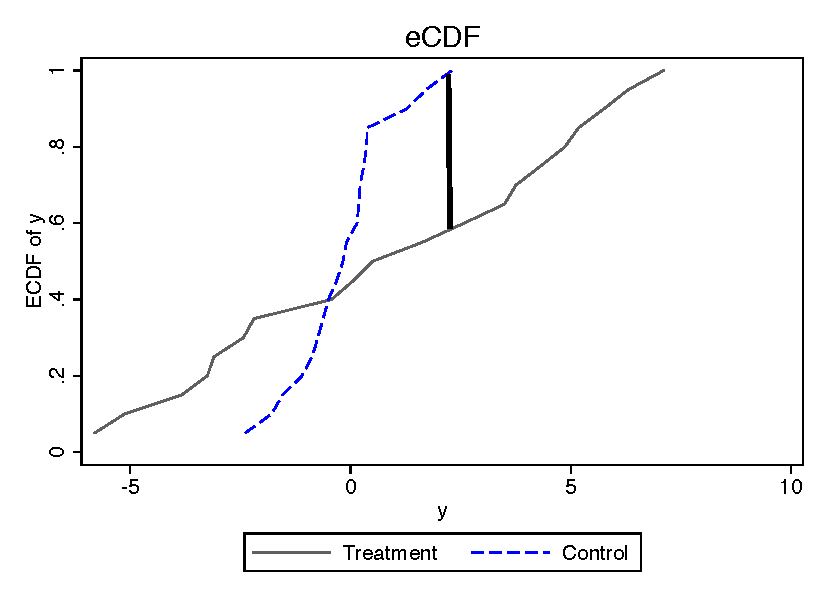
\includegraphics[scale=0.8]{./lecture_includes/ecdf.pdf}     
	\end{figure}
	
\end{frame}




\begin{frame}{Small vs. Modest Sample Sizes are non-trivial}

Computing the exact randomization distribution is not always feasible (Wolfram Alpha)
\begin{itemize}
\item $N=6$ and $N_T=3$ gives us 20 assignment vectors
\item $N=8$ and $N_T=4$ gives us 70 assignment vectors
\item $N=10$ and $N_T=5$ gives us 252 assignment vectors
\item $N=20$ and $N_T=10$ gives us 184,756 assignment vectors
\item $N=50$ and $N_T=25$ gives us 1.2641061$\times 10^{14}$ assignment vectors
\end{itemize}
Exact $p$ calculations are not realistic bc the number of assignments explodes at even modest size

\end{frame}



\begin{frame}{Approximate p-values}

These have been ``exact'' tests when they use every possible combination of $D$ 
	\begin{itemize}
	\item When you can't use every combination, then you can get \emph{approximate} p-values from a simulation (TBD)
	\item With a rejection threshold of $\alpha$ (e.g., 0.05), randomization inference test will falsely reject less than 100$\times \alpha$\% of the time
	\end{itemize}

\end{frame}
\begin{frame}{Approximate $p$ values}

\begin{itemize}
\item Use simulation to get approximate $p$-values
	\begin{itemize}
	\item Take $K$ samples from the treatment assignment space
	\item Calculate the randomization distribution in the $K$ samples
	\item Tests no longer exact, but bias is under your control (increase $K$)
	\end{itemize}
\item Imbens and Rubin show that $p$ values converge to stable $p$ values pretty quickly (in their example after 1000 replications)
\end{itemize}

\end{frame}


\begin{frame}{Thornton's experiment}

\begin{table}[htbp]\small\index{starrandom}
\centering
\begin{tabular}{lcccc}
\toprule
ATE & Iteration & Rank & $p$ & no. trials \\
\midrule
0.45 	 & 1 & 1 & 0.01 & 100\\
0.45 	 & 1 & 1 & 0.002 & 500\\
0.45 	 & 1 & 1 & 0.001 & 1000\\
\bottomrule
\end{tabular}
\caption{Estimated $p$-value using different number of trials.}
\label{tab:starrandom}
\end{table}

\end{frame}

\begin{frame}{Including covariate information}

\begin{itemize}
\item Let $X_i$ be a pretreatment measure of the outcome
\item One way is to use this as a gain score: $Y^{d'} = Y_i^d - X_i$
\item Causal effects are the same $Y^{1i} - Y^{0i} = Y_i^1 - Y_i^0$
\item But the test statistic is different:
\begin{eqnarray*}
T_{gain} = \bigg | ( \overline{Y}_T - \overline{Y}_C ) - (\overline{X}_T - \overline{X}_C ) \bigg |
\end{eqnarray*}
\item If $X_i$ is strongly predictive of $Y_i^0$, then this could have higher power
	\begin{itemize}
	\item $Y_{gain}$ will have lower variance under the null
	\item This makes it easier to detect smaller effects
	\end{itemize}
\end{itemize}

\end{frame}

\begin{frame}{Regression in RI}

\begin{itemize}
\item We can extend this to use covariates in more complicated ways
\item For instance, we can use an OLS regression:
\begin{eqnarray*}
Y_i = \alpha + \delta D_i + \beta X_i +  \varepsilon
\end{eqnarray*}
\item Then our test statistic could be $T_{OLS} = \widehat{\delta}$
\item RI is justified even if the model is wrong
	\begin{itemize}
	\item OLS is just another way to generate a test statistic
	\item The more the model is ``right'' (read: predictive of $Y_i^0$), the higher the power $T_{OLS}$ will have
	\end{itemize}
\item See if you can do this in Thornton's dataset using the loops and saving the OLS coefficient (or just use \texttt{ritest})
\end{itemize}

\end{frame}

\begin{frame}{Concluding remarks}

\begin{itemize}
\item Randomization inference is very common, particularly useful you don't want to make strong assumptions (parametric free)
\item It's an area of continual examination by statisticians and econometricians, both in the experimental design and the quasi-experimental design
\item We will use it primarily in my workshops with synthetic control, but it's going to be one you encounter and valued because of the non-parametric nature of it
\end{itemize}

\end{frame}



\end{document}
\begin{frame}{Angrist and Imbens and the 1990s}

  \begin{itemize}
    \item Angrist writes a dissertation using randomized instruments (Vietnam draft), goes to Harvard, overlaps with Imbens for a year, they are mentored by Gary Chamberlain, work with Don Rubin, write their famous LATE paper
    \item Chamberlain recommends potential outcomes framework over a different one that had been used at that time (latent index) and that seems to make the work more generally attractive (like to Rubin)
    \item Let's spend twenty minutes listening to them
  \end{itemize}

\end{frame}

\begin{frame}{Angrist, Imbens and Harvard}


  Josh Angrist on the negative results at the time (10 min)

  \url{https://youtu.be/ApNtXe-JDfA?t=1885}


  \bigskip
  Guido Imbens on the reception of their work (10 min)

  \url{https://youtu.be/cm8V65AS5iU?t=799}

\end{frame}
